%\documentclass[aps,prb,twocolumn,showpacs]{report}
\documentclass[11pt]{report}

\usepackage{graphicx}
\usepackage{amsfonts}
\usepackage{amssymb}
\usepackage{amsmath}
\usepackage{mathrsfs}
\usepackage{braket}
\usepackage{epstopdf}
\usepackage{geometry}
\geometry{margin=1in}

\def\avg#1{\langle#1\rangle}
\def\v#1{\mathbf{#1}}
\def\Re {\mbox{Re}}
\def\Im {\mbox{Im}}
\def\tr{\mbox{tr}}
\def\nn{\nonumber}
\def\pp{\parallel}
\def\ket#1{\vert #1 \rangle}
\def\bra#1{\langle #1 \vert}
\def\me#1#2#3{\langle #1 \vert #2 \vert #3 \rangle}
\def\Br{\mathbf{r}}

\newcommand{\kp}{k_{+}}
\newcommand{\ki}{k_{-}}
\newcommand{\idz}{i\partial_z}
\newcommand{\kperp}{\mathbf{k}_\parallel}

\title{Thesis Proposal: \\Nanostructures with Topological Insulators}
\author{Mahmoud Lababidi}

\begin{document}

\maketitle
\tableofcontents

\chapter{Introduction}
\section{Overview}
In this proposal I will have four basic parts that break down the why, how and what I propose to do in my research for my thesis. I begin by presenting a brief introduction to topological insulators which can be skipped for brevity if one is already familiar with the subject. This introduction will not be as detailed as many papers on the subject but should suffice for understanding the proposed actions in this proposal. Then I will highlight some novel and interesting physics that have been spurred from the TI. This is simply to motivate the projects that I have and will work on. Next, I will present work already completed and in progress. Lastly, I will present the next projects that I aim to complete towards my research. 


\section{Motivation and Background}
Topological Insulators (TIs) are a new form of matter that have robust conducting metallic surface states while the bulk is an insulator. The surface is so vastly different from the bulk, that it can be seen as a playground of new properties never seen before. One such novel property is that the surface is host to Dirac Fermions which behave relativistically and massless-like. Such particle behavior was predicted by Paul Dirac. The first experiment that demonstrated this prediction was done on graphene, a very similar cousin to the TI. These particles are identified as  Dirac Fermions because they obey the Dirac equation which models relativistic (near speed of light) particles. These massless relativistic Fermions, demonstrate a direct linear relationship between the energy (E) and their quantized momentum (k), $E=\pm\hbar v k$. This peculiar energy relationship is uncommon in  materials. 

This low energy linear dispersion deviates from the simple yet exotically elegant  $k\cdot p$ Hamiltonian
\begin{equation}
H=\vec{\sigma}\cdot \vec{k}-\mu=\sigma_x k_x + \sigma_y k_y - \mu
\end{equation}
on the surface is host to electrons that have their spin and momentum direction locked. This locking is completely due to the spin-orbit coupling that is similarly found in Rashba spin-orbit coupled materials.

The insulator component exists due to the fact that the SOC actually causes the bulk of the material to have a fully gapped energy spectrum while the robust surface Hamiltonian is a result of the surface boundary. This robustness is also a result of the non-trivial topological nature of the material. These surface states are not an accident due to possible band crossing but rather a definition of a topological phase transition from the bulk to the boundary.

\section{Majorana Particles}
TIs have gained much notoriety for a variety of new physics. Such physics include the proposal to generate Majorana particles, which are non-Abelian, through the use of superconductors in proximity; interesting conductance on the surface due to the Dirac-like Hamiltonian and spin (eg Klein Tunneling); and the possibility of new topological phases of materials.



\section{Spintronics}
Electronic or spintronic devices based on topological insulators will almost inevitably involve metal as measurement probes or functioning components \cite{yokoyama09}. This motivates us to study the local spectrum near the interface between a metal (M) and a topological insulator (TI). For a metal-ordinary semiconductor junction with good contact, it is well known that the metallic Bloch states penetrate into the semiconductor as evanescent waves localized at the interface (for energies within the band gap). Such interface states are known as metal induced gap states (MIGS) \cite{heine65,cohen}. They play an important role in controlling the junction properties, e.g., by pinning the semiconductor Fermi level to determine the Schottky barrier height \cite{tersoff}, a key parameter of the junction.



\chapter{Metal to Topological Insulator Scattering}


We compute the spin-active scattering matrix and the local spectrum at the interface between a metal and a three-dimensional  topological band insulator. We show that there exists a critical incident angle at which complete (100\%) spin flip reflection occurs and the spin rotation angle jumps by $\pi$. We discuss the origin of this phenomena, and systematically study
the dependence of spin-flip and spin-conserving scattering amplitudes on
the interface transparency and metal Fermi surface parameters.
The interface spectrum contains a well-defined Dirac cone in the tunneling limit, and smoothly evolves into a continuum of metal induced gap states for good contacts. We also investigate the complex band structure of Bi$_2$Se$_3$.

\section{Introduction}
Recently discovered three dimensional topological band insulators \cite{fu07,moore,roy}, such as Bi$_{1-x}$Sb$_x$ \cite{Hsieh2008} and Bi$_2$Se$_3$ \cite{Xia09,zhang2009,Chen09}, are spin-orbit coupled crystal solids with a bulk gap but protected gapless surface states. The low energy excitations at the surface are helical Dirac fermions, i.e., their spin and momentum are entangled (locked) \cite{Hsieh2009}. The charge and spin transport on the surface of a topological insulator
are intrinsically coupled \cite{burkov}.
This makes these materials a promising new platform for spintronics. In addition, heterostructures involving topological insulator, superconductor, and/or ferromagnet have been predicted to show a remarkable array of novel spectral and transport properties (for review
see Ref. \cite{today,rmp,Qi-zhang-rev}). 

Electronic or spintronic devices based on topological insulators will almost inevitably involve metal as measurement probes or functioning components \cite{yokoyama09}. This motivates us to study the local spectrum near the interface between a metal (M) and a topological insulator (TI). For a metal-ordinary semiconductor junction with good contact, it is well known that the metallic Bloch states penetrate into the semiconductor as evanescent waves localized at the interface (for energies within the band gap). Such interface states are known as metal induced gap states (MIGS) \cite{heine65,cohen}. They play an important role in controlling the junction properties, e.g., by pinning the semiconductor Fermi level to determine the Schottky barrier height \cite{tersoff}, a key parameter of the junction.

The local spectrum at the M-TI junction is intimately related to the spin-active scattering of electrons at the M-TI interface. In this paper, we systematically study the evolution of the scattering matrix and the interface spectra
with the junction transparency and metal Fermi surface parameters. 
%by exploiting the {\it complex band structure} of topological insulators, which describes the decaying (rather than propagating Bloch wave) solutions of the crystal Hamiltonian.
The scattering matrix \cite{mrs} we obtain here also forms the basis to investigate the details of the superconducting proximity effect near the superconductor-TI interface \cite{stan}, which was shown by Fu and Kane to host Majorana fermions \cite{majorana}.

The scattering at the M-TI interface differs significantly from its two dimensional analog, the interface between a metal and a quantum spin Hall (QSH) insulator studied by Tokoyama et al \cite{yokoyama09}. They predicted a giant spin rotation angle $\alpha\sim \pi$ and interpreted the enhancement as resonance with the one-dimensional helical edge modes. By contrast, for M-TI interface we predict a critical incident angle at which complete spin flipping occurs and the spin rotation angle jumps by $\pi$. We will explain its origin, {in particular its relation to the surface helical Dirac spectrum}, and discuss its spintronic implications.

This paper is organized as follows. 
We will first compute the scattering matrix using a $\mathbf{k\cdot p}$ continuum model 
by matching the envelope wave functions at the M-TI interface. This simple calculation is easy to understand, 
and it brings out
the main physics of our problem. Along the way, we will discuss the complex band structure of Bi$_2$Se$_3$,
 which describes the decaying (rather than propagating Bloch wave) solutions of the crystal Hamiltonian.
The various caveats of this calculation 
are then remedied by considering a much more general lattice model. Most importantly, it enables us to 
track how the scattering matrix and interface spectrum change with interface transparency. It also sheds light on
the origin of perfect spin-flip scattering at the critical angle.
We will show that the results obtained from these two complementary methods are consistent with each.

\section{Model Hamiltonian and Complex Band Structure}

We consider Bi$_2$Se$_3$ as a prime example of 3D strong topological insulators. Its low energy $\mathbf{k\cdot p}$ Hamiltonian was obtained by Zhang et al \cite{zhang2009},
\[
\hat{H}_{TI}(\v{k})=\epsilon_0(\v{k})\hat{1}+\sum_{\mu=0}^{3}d_\mu(\v{k})\hat{\Gamma}_\mu.
\]
Here $d_0(\v{k})=M-B_1k^2_z-B_2(k_x^2+k_y^2)$, $d_1(\v{k})=A_2 k_x$, $d_2(\v{k})=A_2 k_y$, $d_3(\v{k})=A_1 k_z$, and $\epsilon_0(\v{k})=C+D_1k_z^2+D_2(k_x^2+k_y^2)$. The numerical values of $M$, $A$, $B$, $C$, $D$ are given in Ref. 
\cite{zhang2009}.
We choose the basis ($\ket{+\uparrow}$, $\ket{+\downarrow}$, $\ket{-\uparrow}$,$\ket{-\downarrow}$), where $\pm$ labels the hybridized $p_z$ orbital with even (odd) parity \cite{zhang2009}. The Gamma matrices are defined as
$\hat{\Gamma}_0=\hat{\tau}_3\otimes \hat{1}$, $\hat{\Gamma}_i=\hat{\tau}_1\otimes \hat{\sigma}_i$, with
$\hat{\tau}_i$ ($\hat{\sigma}_i$) being the Pauli matrices in the orbital (spin) space.
The chemical potential of as-grown Bi$_2$Se$_3$ crystal actually lies in the conduction 
band \cite{Hsieh2009}. By hole doping \cite{Hsieh2009} 
or applying a gate voltage \cite{gate}, the chemical potential can be tuned inside 
the gap. The system is well described by $H_{TI}$ (note that energy zero is set as 
in the middle of the band gap).

In this section, we first adopt a rather artificial model for metals with negligible 
spin-orbit coupling. It is
obtained by turning off the spin-orbit interaction (setting $d_\mu=0$ for $\mu$=1,2,3) 
in $H_{TI}$ and shifting the Fermi level into 
the conduction band. The result is spin-degenerate two-band Hamiltonian
\[
\hat{H}_M(\v{k})=[\epsilon_0(\v{k})-E_F]\hat{1}+d_0(\v{k})\hat{\Gamma}_0.
\]
Its band structure, schematically shown in Fig. 1(b), consists of two oppositely dispersing bands 
(the solid and dash line). $E_F$ is tuned to be much higher than the band crossing point, so
the scattering properties of low energy electrons near the Fermi surface are 
insensitive to the band crossing at high energies. This claim will be verified later using a
more generic model for the metal. A similar model was used in the study of metal-QSH interface \cite{yokoyama09}.

%%%%%%%%%%%%%%%%%%%%%%%%%%

\begin{figure}
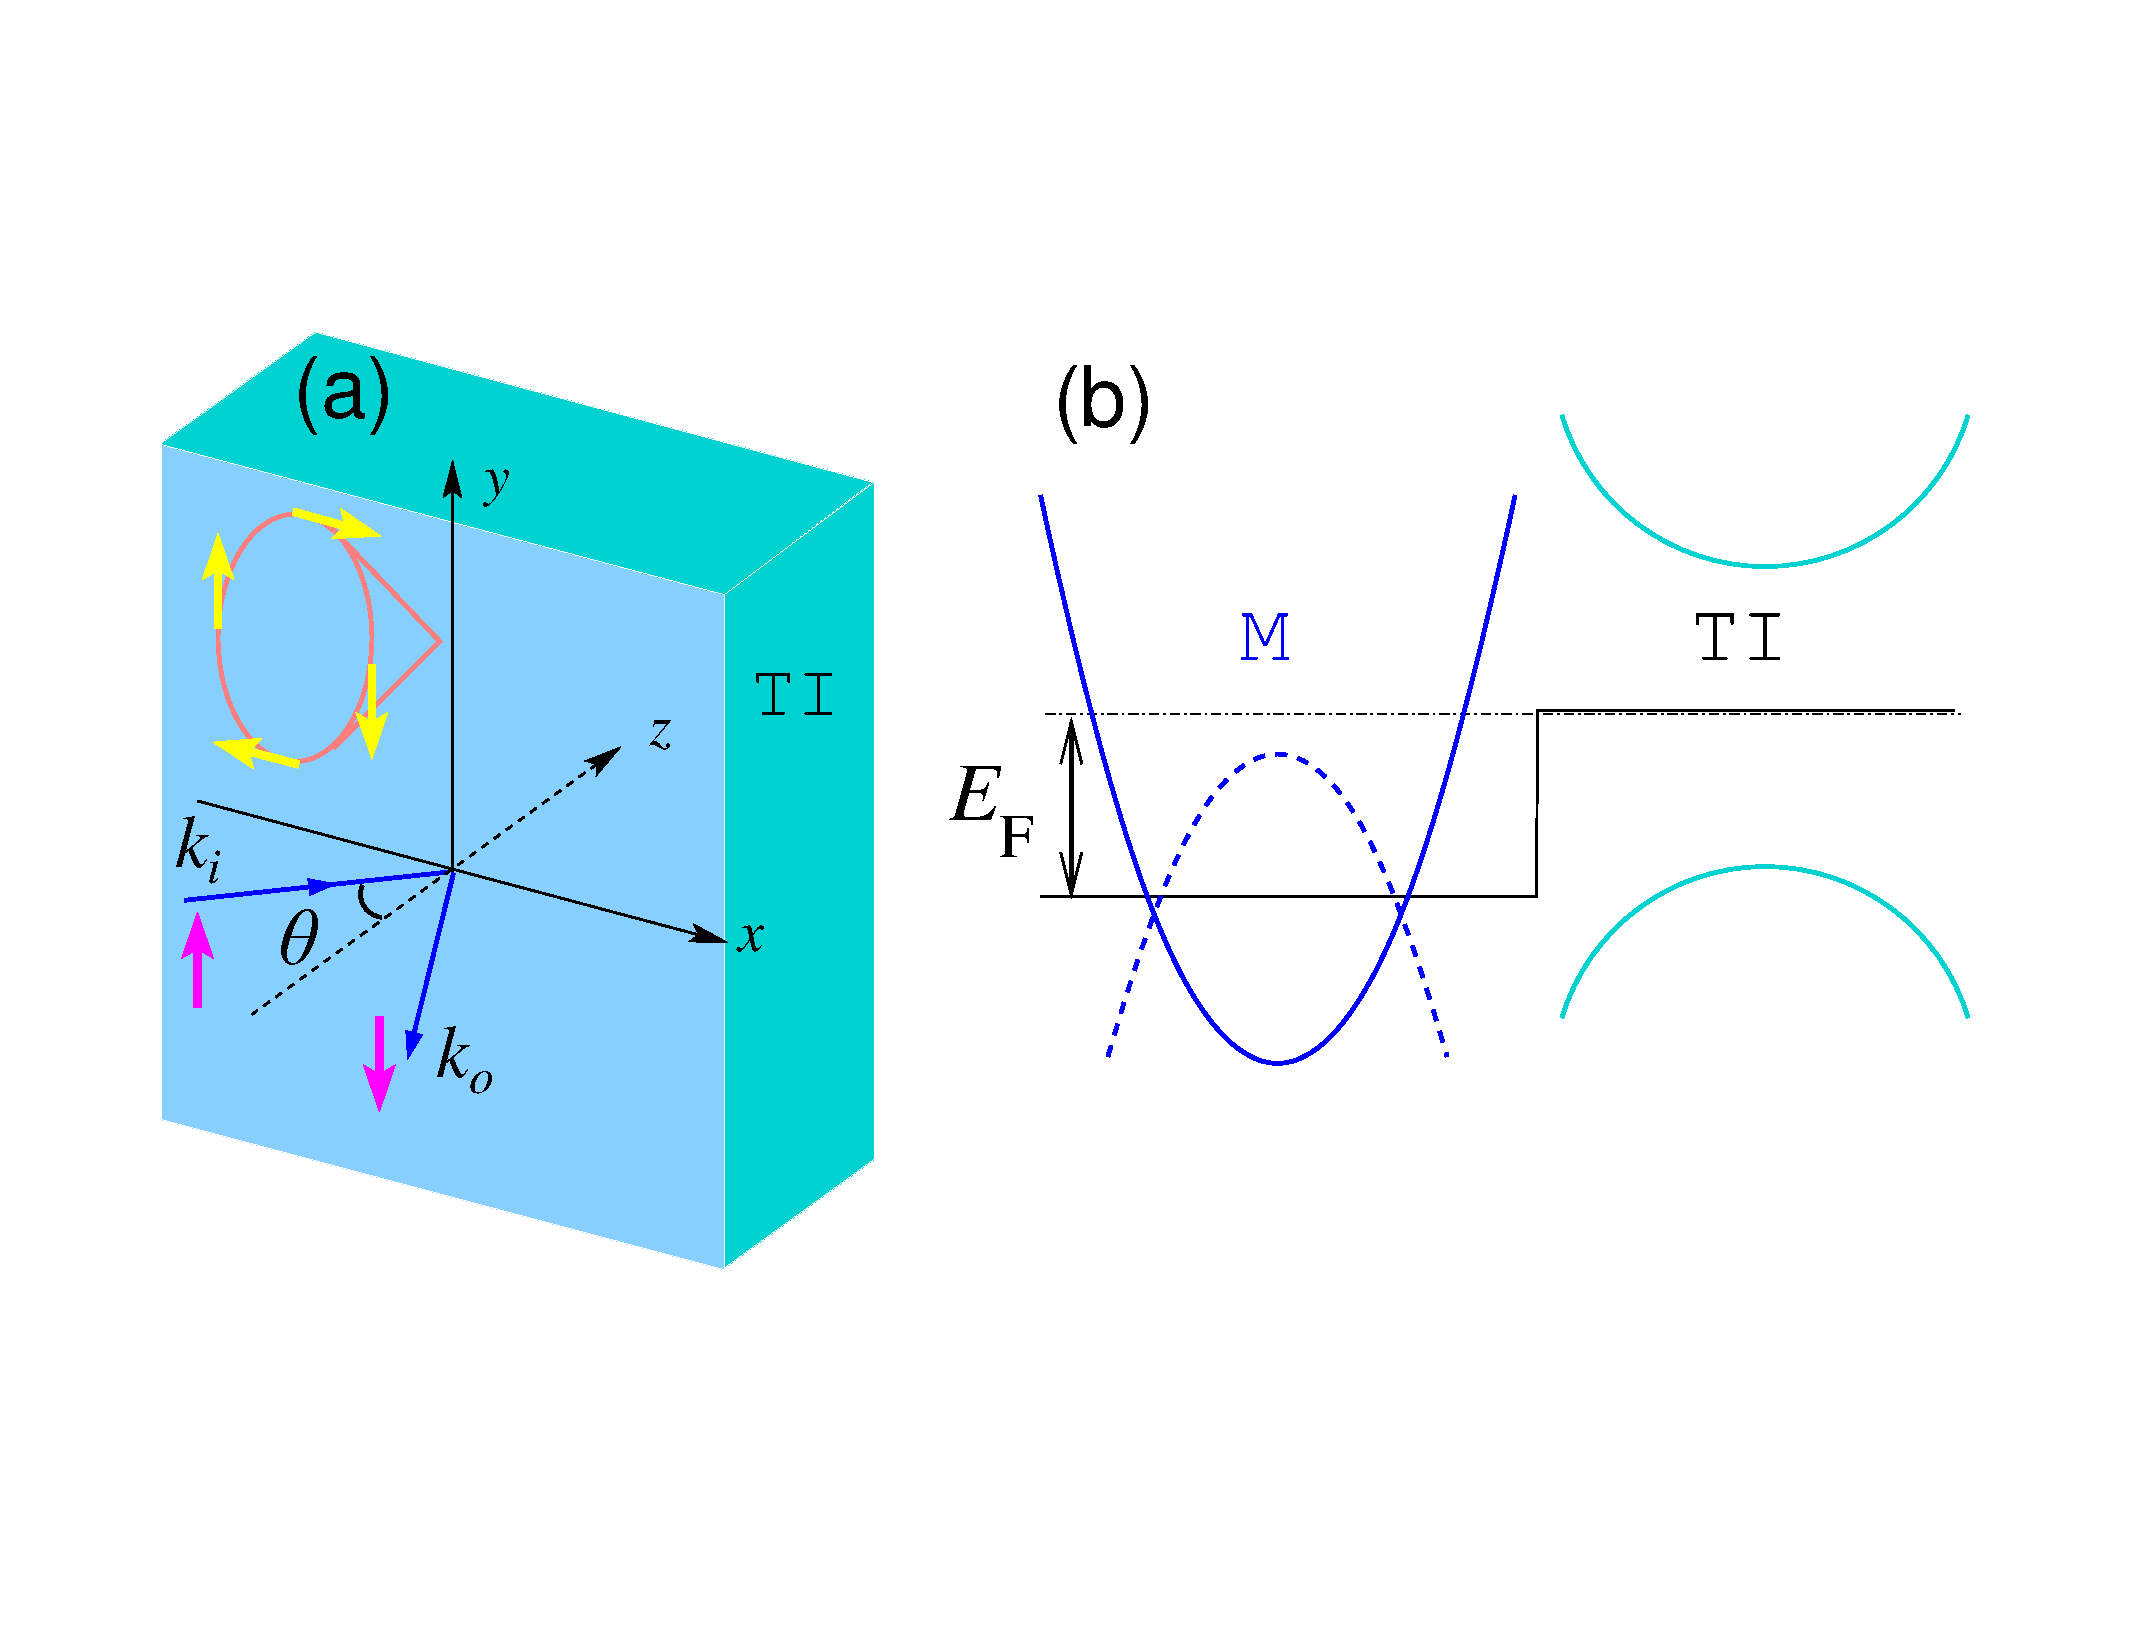
\includegraphics[width=3.4in]{geometry.pdf}
\caption{(a) Scattering geometry at a metal (M)-topological insulator (TI) interface.
(b) Schematic band structure of the metal (modeled by $\hat{H}_M$) and topological insulator.
}
\end{figure}
%%%%%%%%%%%%%%%%%%%%%%%%%%


Matching the wave functions of two dissimilar 
materials (such as Au and Bi$_2$Se$_3$) at interface is in general 
complicated within the $\mathbf{k\cdot p}$ formalism, because the envelope wave functions 
on either side are defined using different basis (see Ref. \cite{bc} and reference therein). 
For the particular model $H_M$, however, such complication
is circumvented. Then, then wave functions at the metal-TI interface ($z=0$) satisfy the Ben-Daniel 
and Duke boundary condition \cite{duke}, 
\[
\hat{\Phi}_M=\hat{\Phi}_{TI}, \;\;\; \hat{v}_M \hat{\Phi}_M = \hat{v}_{TI}\hat{\Phi}_{TI}.
\]
Here $\hat{\Phi}_i$ is the four-component wave function, and 
the velocity matrix $\hat{v}_{i}=\partial \hat{H}_i/\partial k_z$, $i\in \{M, TI\}$. 
Such boundary condition assumes good atomic contact between two materials.

We are interested in energies below the band gap of TI, so 
$\hat{\Phi}_{TI}$ is evanescent in nature and only penetrates into TI 
for a finite length. Such localized (surface or interface) 
states inside topological insulator can be treated within the $\mathbf{k\cdot p}$ formalism 
using the theory of {\it complex band structures}, pioneered by Kohn \cite{kohn59}, Blount \cite{blount62}, 
and Heine \cite{heine63} et al. 
The main idea is to allow the crystal momentum to be complex and analytically continue
$H_{TI}(\v{k})$ to the complex $\v{k}$ plane. 
While the extended Bloch waves are the eigen states of $H_{TI}(\v{k})$ for real $\v{k}$, 
eigen functions of $H_{TI}(\v{k})$ for complex $\v{k}$ describe localized states. Together they
form a complete basis to describe crystals of finite dimension. 

%%%%%%%%%%%%%%%%%%%%%%%%%%
\begin{figure}
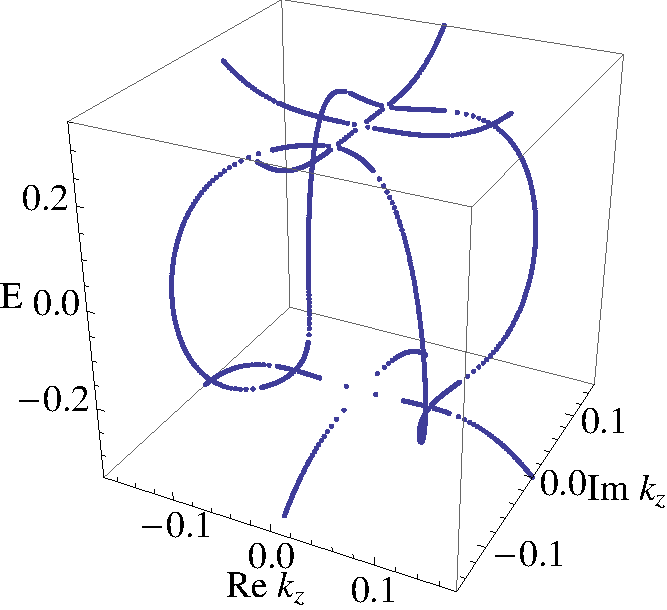
\includegraphics[width=1.7in]{f2.pdf}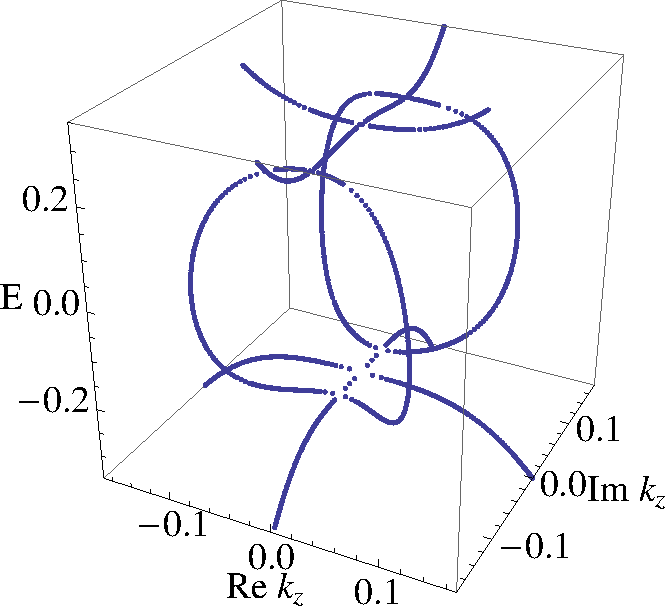
\includegraphics[width=1.7in]{f4.pdf}
\caption{The complex band structure
of topological insulator described by $\hat{H}_{TI}(\v{k})$ 
for $k_y=0$, $k_x=0.02$ (left) and $0.04$ (right). $E$ is measured in eV, and $k$ in $\AA^{-1}$.
Subgap states with complex $k_z$ represent evanescent waves. 
The topology of  real lines \cite{heine63}  changes as $k_x$ is increased.  
}
\end{figure}
%%%%%%%%%%%%%%%%%%%%%%%%%%

In our scattering problem, we have to find all eigen states of $H_{TI}(\v{k})$ with energy $E$ and 
wave vector $\v{k}=(k_x,k_y,\tilde{k}_z)$, where $k_x$ and $k_y$ are given and real, but $\tilde{k}_z$ is 
complex and unknown. For a general $\mathbf{k\cdot p}$ Hamiltonian such as $\hat{H}_{TI}$, 
we follow Chang and Schulman \cite{chang82} to rewrite it as
\[
\hat{H}_{TI}=\hat{h}_0(k_x,k_y)+\hat{h}_1 \tilde{k}_z+\hat{h}_2\tilde{k}^2_z,
\]
where $\hat{h}_1=A_1\hat{\Gamma}_3$, and $\hat{h}_2=-B_1\hat{\Gamma}_0$. 
Then the eigen equation $(\hat{H}_{TI}-E\hat{1})\hat{\phi}=0$ can be reorganized into an 
eigen value problem for $\tilde{k}_z$,
\[
\left(
\begin{array}{ll}
  0 & 1   \\
  -\hat{h}_2^{-1}(\hat{h}_0-E\hat{1}) & -\hat{h}_2^{-1}\hat{h}_1
  \end{array}
\right)
\left(
\begin{array}{l}
  \hat{\phi}   \\
  \hat{\phi}'  
\end{array}
\right)
=\tilde{k}_z \left(
\begin{array}{l}
  \hat{\phi}   \\
  \hat{\phi}'    
\end{array}
\right).
\]
%%% note: these details can be omitted to save space 
Then all possible values of $\tilde{k}_z$ can be obtained for given incident parameter $E$, $k_x$, and $k_y$. 
For the anisotropic Dirac Hamiltonian $H_{TI}(\v{k})$, the energy eigenvalues can be obtained 
analytically \cite{qi_field}, which allows for an analytical solution of the complex band structure.

For $E$ within the gap, there are in general 4 pairs of complex solution of $\tilde{k}_z$, for if $\tilde{k}_z$ is a solution so is $\tilde{k}^*_z$. 
We label those with positive imaginary parts with $\{\tilde{k}^\nu_z\}$, and the corresponding wave function $\{\hat{\phi}^\nu \}$, $\nu=1,2,3,4$. They are decaying solutions in the half space $z>0$. In our model, $\tilde{k}_z$ turns out to be doubly degenerate, as shown in Fig. 2. The wave function inside TI ($z>0$) then has the form
\[
\hat{\Phi}_{TI}=\sum_{\nu} t_\nu e^{i\tilde{k}^\nu_z z} \hat{\phi}_\nu.
\]

\section{Scattering Matrix from Wave-Function Matching} 

To set the stage for discussing scattering off a topological insulator, it is instructive to recall the generic features of elastic scattering of electrons by a heavy ion with spin-orbit interaction. This classical problem was solved by Mott, and known as {\it Mott scattering}. 
%It is being used, for example, to measure the spin polarization of photo electrons in spin-resolved ARPES. 
% Spin-orbital coupling amounts to a momentum dependent magnetic field $\mathbf{B}(\mathbf{k})$, which causes the spin of incident electron to precess. 
The scattering matrix has the general form \cite{mott}
\[
\hat{S}_{Mott}=u\hat{1}+w\hat{\boldsymbol{\sigma}}\cdot (\mathbf{k}_{i}\times \mathbf{k}_{o}),
\]
where $\mathbf{k}_{i}$ and $\mathbf{k}_{o}$ are the incident and outgoing momentum respectively, $\hat{\boldsymbol{\sigma}}$ is the Pauli matrix, and $u,w$ depend on the scattering angle. It is customary to
define the spin-flip amplitude $f=S_{21}$, and spin-conserving amplitude $g=S_{11}$. 
Both $f$ and $g$ are complex numbers, their relative phase defines the {\it spin rotation angle} $\alpha=\mathrm{Arg}(g^*f)$.
One immediately sees that for back scattering, $\hat{S}_{Mott}=u\hat{1}$, so there is no spin flip, $f=0$. As we will show below, this also holds true for scattering off TI.

Now consider an electron coming from the metal 
with momentum $\v{k}$ incident on the M-TI interface located at $z=0$, 
as schematically shown in Fig. 1(a). 
We assume the interface is 
translationally invariant, so the transverse momentum $\v{k}_{\parallel}=(k_x,k_y)$ is 
conserved, and the energy $E$ of the electron 
lies within the band gap of TI. Then, only total reflection 
is possible, but the spin-orbit coupling inside TI acting like a $\v{k}$-dependent magnetic field rotates the spin of the incident particle. The scattering (reflection) matrix has the form
\[
\hat{S}(\v{k})=\left(
\begin{array}{ll}
  g & \bar{f}   \\
  f & \bar{g}
  \end{array}
\right),
\]
where $|g|^2+|f|^2=1$. 
Our goal is to find the dependence of the scattering amplitudes $f,g$ 
on $\v{k}$, or equivalently, on energy $E$ and 
incident angle $\theta$. From time-reversal symmetry, 
$\bar{f}(E,\theta)=f(E,-\theta)$ and $\bar{g}(E,\theta)=g(E,-\theta)$.
We shall show that
$f(\v{k}_{\parallel})=-f(-\v{k}_{\parallel}$),
$g(\v{k}_{\parallel})=g(-\v{k}_{\parallel}$). So 
$f$ is an odd function of $\theta$, while $g$ is even in $\theta$.  
Since our problem can be viewed as coherent multiple scattering from a lattice 
array of Mott scatters occupying half the space, we will refer to
spin-active scattering at the metal-TI interface as Mott scattering.

Consider a spin up electron from the conduction band of the metal 
with momentum $\v{k}$ and energy $E=
\epsilon_0(\v{k})-E_F-d_0(\v{k})$ lying within the band gap of TI.
The wave function inside the metal ($z<0$) has the form
\[
\hat{\Phi}_M=(r_1e^{-ik'_{z} z},r_2e^{-ik'_{z}z},e^{ik_{z}z}+r_3 e^{-ik_{z}z} ,r_4 e^{-ik_{z}z})^{\mathrm{T}},
\]
up to the trivial $e^{i(k_x x+k_y y)}$ and renormalization factor.
Here $k_z=\hat{z}\cdot\v{k}$, and $\{r_i\}$ are the reflection amplitudes. We identify 
the spin flip amplitude $f=r_4$ and the spin-conserving amplitude $g=r_3$. Note that 
there is no propagating mode at energy $E$ available in the valence band 
for the reflected electron. So $k'_z$ is purely imaginary. 
%
At such energy, there is no propagating mode available in TI. We have discussed the 
evanescent wave function $\hat{\Phi}_{TI}$ in the previous section.
With $\hat{\Phi}_{M}$ and $\hat{\Phi}_{TI}$, we solve the boundary condition at $z=0$ 
to obtain $r_\nu, t_\nu$ and the scattering matrix $S$. 

Fig. 3 shows the magnitude and phase of $f$ and $g$ versus the incident angle $\theta$ for $E=0.1$eV, with $E_F$ set to be 0.28eV. At normal incidence, $\theta=0$, spin flip scattering
is forbidden as in the single-ion Mott scattering. With increasing $\theta$ the magnitude of $g$ drops continuously. At a critical angle $\theta_c$, $|g|$ drops to zero and we have perfect (100\%) spin flip reflection.
At the same time, the spin rotation angle $\alpha$ (the relative phase between $f$ and $g$)
jumps by $\pi$.

It is tantalizing to think of what happens at $\theta_c$ as resonant scattering
with the helical surface mode of the TI. This however is problematic.
We are considering good contacts at which the wave functions of the two materials hybridize strongly. 
Surface mode is preempted by MIGS. Indeed, we checked that the corresponding critical 
transverse momentum $k_\parallel$ depends only weakly on $E$. This is at odds with
the linear dispersion of the TI surface mode, $E=A_2k_\parallel$ \cite{zhang2009}. To gain better
understanding, we now switch to a lattice model to systematically study the role of interface 
transparency and metal Fermi surface parameter ($E_f, k_f, v_f$) on the scattering matrix. 



%%%%%%%%%%%%%%%%%%%%%%%%%%
\begin{figure}
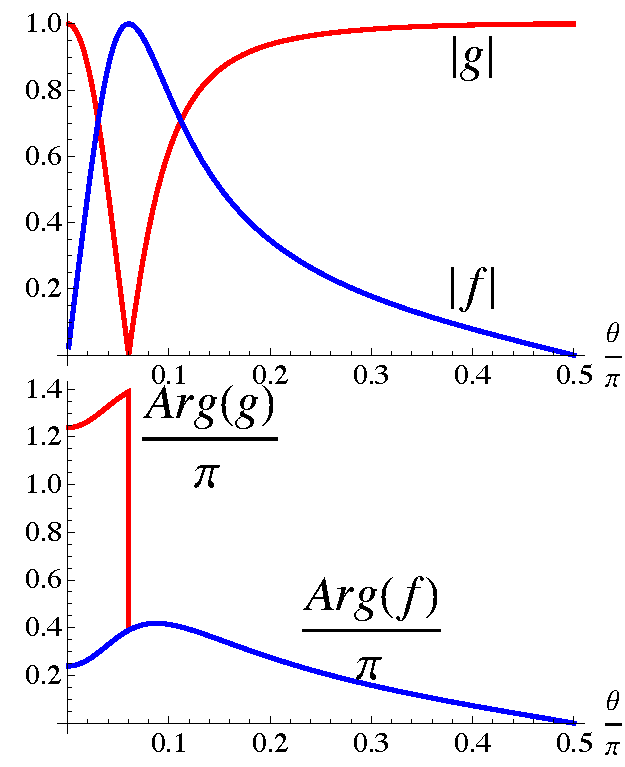
\includegraphics[width=2.5in]{scatt.pdf}
\caption{ The magnitudes (upper panel) and the phases (lower panel) of the spin-flip 
amplitude $f$ and spin-conserving amplitude $g$ versus the incident angle $\theta$.
$E=0.1$eV, $E_F$=0.28eV. $|g|^2+|f|^2=1$. Arg($g$) and Arg($f$) 
are shifted upward by $\pi$ for clarity.}
\end{figure}
%%%%%%%%%%%%%%%%%%%%%%%%%%

\section{Interface Spectrum and Scattering Matrix from Lattice Green Function} 

We consider a simple lattice model for the M-TI junction.
The topological insulator is modeled by 
a tight binding Hamiltonian on cubic lattice,
\begin{align*}
&\mathscr{H}_R=\sum_{\kp,n}\left\{ 
\hat{\psi}_{\kp,n}^\dagger (b_1\hat{\Gamma}_0-i\frac{a_1}{2}\hat{\Gamma}_3)  \hat{\psi}_{\kp,n+1}+ h.c. \right. \\
&+\left. 
\hat{\psi}_{\kp,n}^\dagger\left[d(\kp)\hat{\Gamma}_0+a_2(\hat{\Gamma}_1\sin k_x +\hat{\Gamma}_2\sin k_y)\right] \hat{\psi}_{\kp,n} \right\} .
\end{align*}
Here $\hat{\psi}=(\psi_{+\uparrow},\psi_{+\downarrow},\psi_{-\uparrow},\psi_{-\downarrow})^\mathrm{T}$ is the annihilation operator, $d(\kp)=M-2b_1+2b_2(\cos k_x+\cos k_y-2)$ with $k$ measured in $1/a$. 
The cubic lattice consists of layers of square lattice stacked in the $z$ direction,
$n$ is the layer index, and $\kp$ is the momentum in the $xy$ plane.
The isotropic version of $\mathscr{H}_R$, with $a_1=a_2$, $b_1=b_2$, was 
studied by Qi et al as a minimal model for 3D topological insulators \cite{qi_field}.
To mimic Bi$_2$Se$_3$, we set the lattice spacing $a=5.2$\AA, which gives the correct unit cell volume, 
and $a_i=A_i/a$, $b_i=B_i/a^2$ for $i=1,2$. Although a crude caricature 
of the real material, $\mathscr{H}_R$ yields the correct gap size and surface dispersion, it also reduces to 
the continuum  $\mathbf{k\cdot p}$ Hamiltonian $\hat{H}_{TI}$ in the small $k$ limit, 
aside from the topologically trivial $\epsilon_0(\v{k})$ term.
 
%%%%%%%%%%%%%%%%%%%%%%%%%%
\begin{figure}
%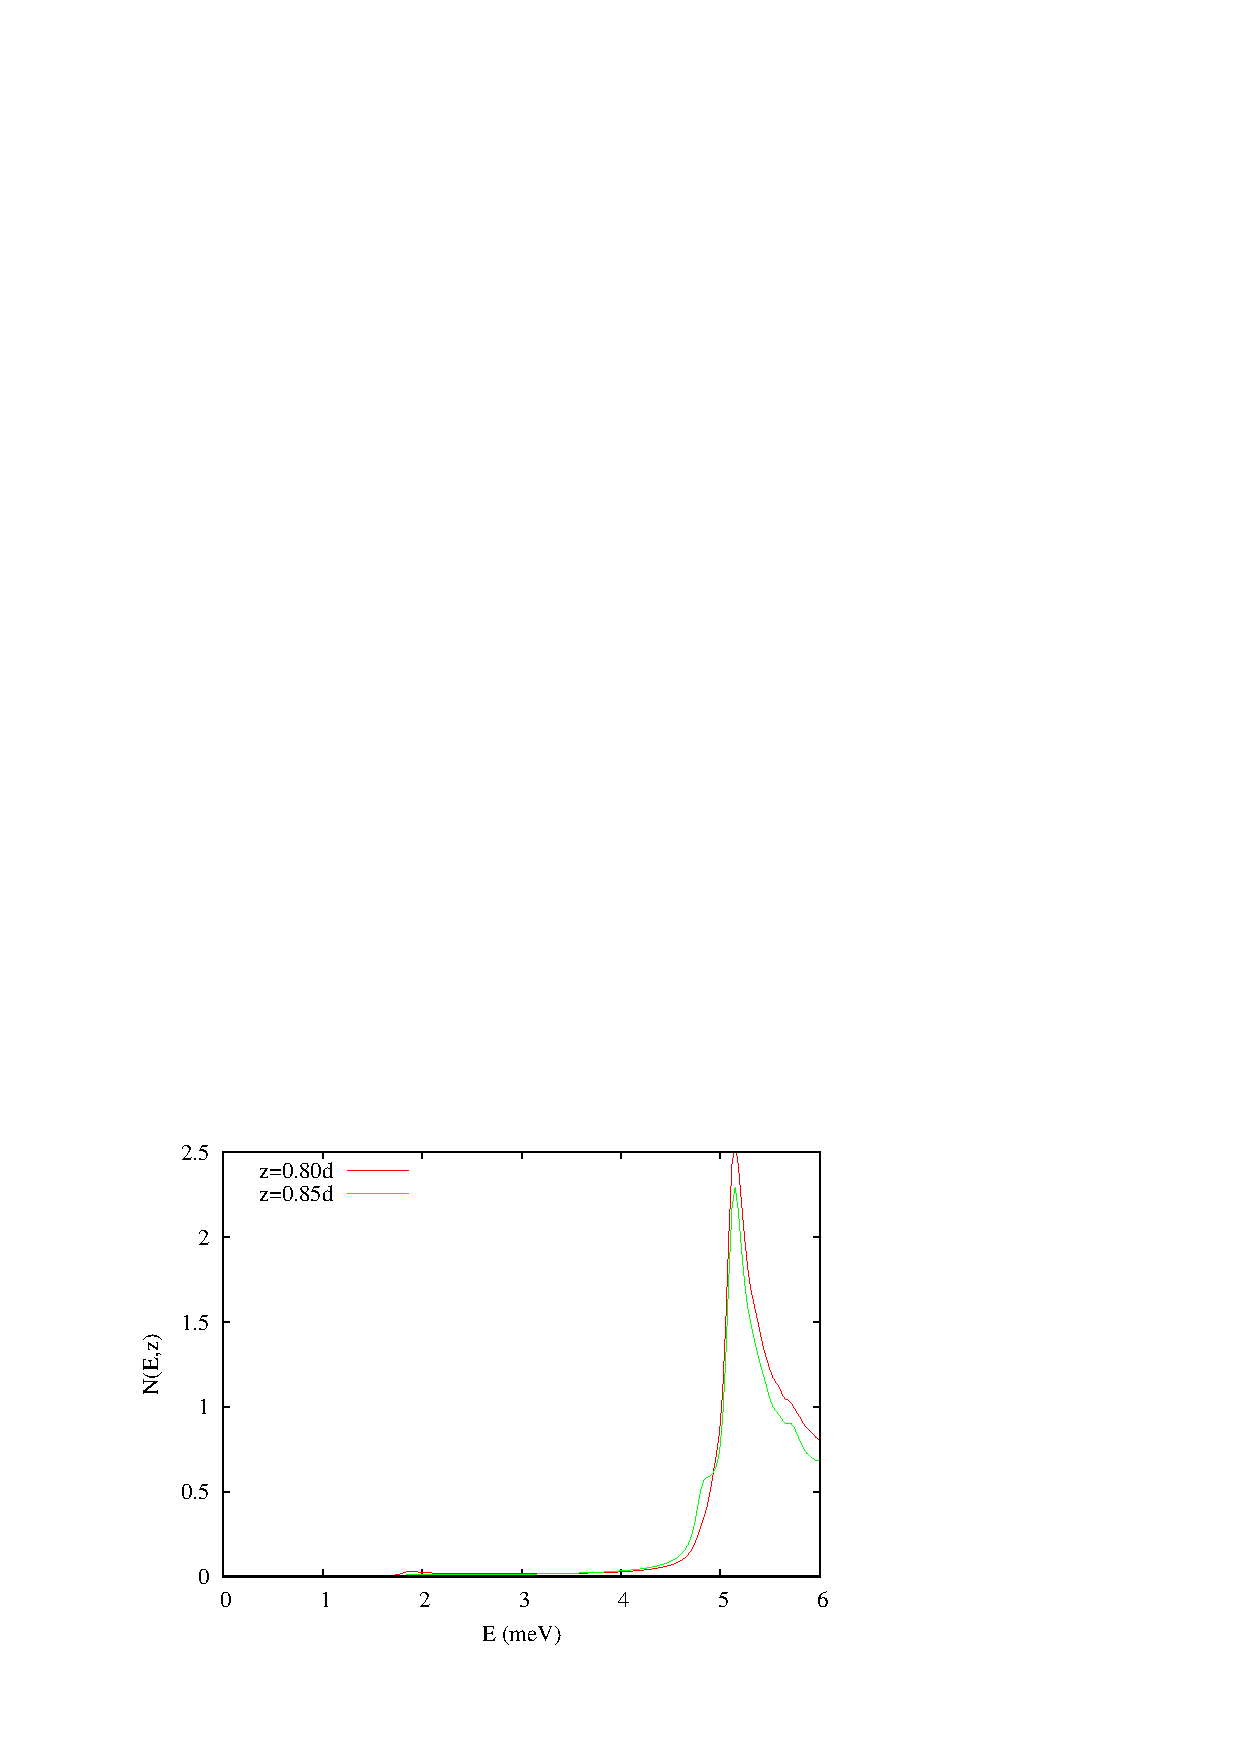
\includegraphics[width=3.4in]{dos.pdf}
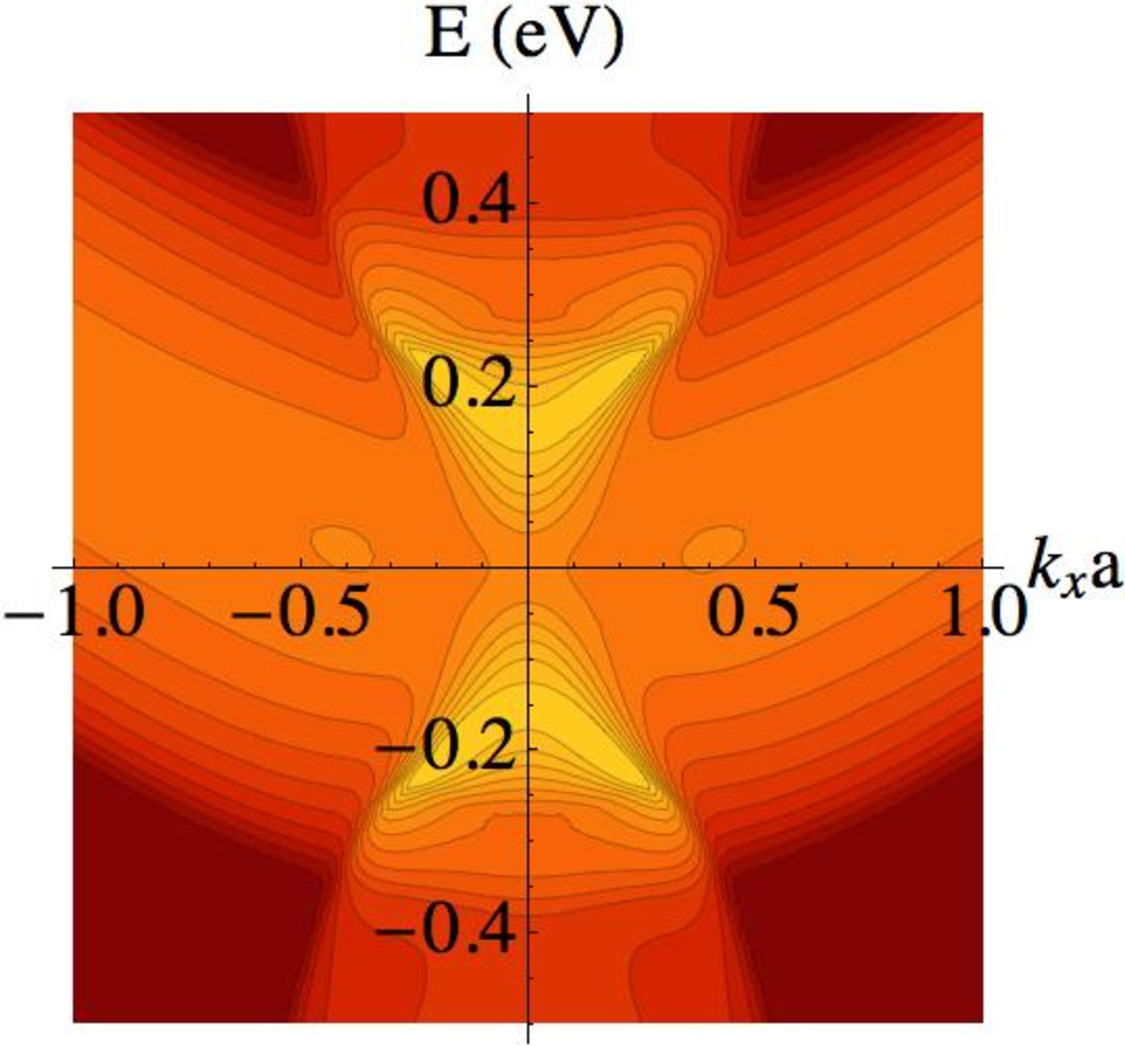
\includegraphics[width=1.7in]{j1.pdf}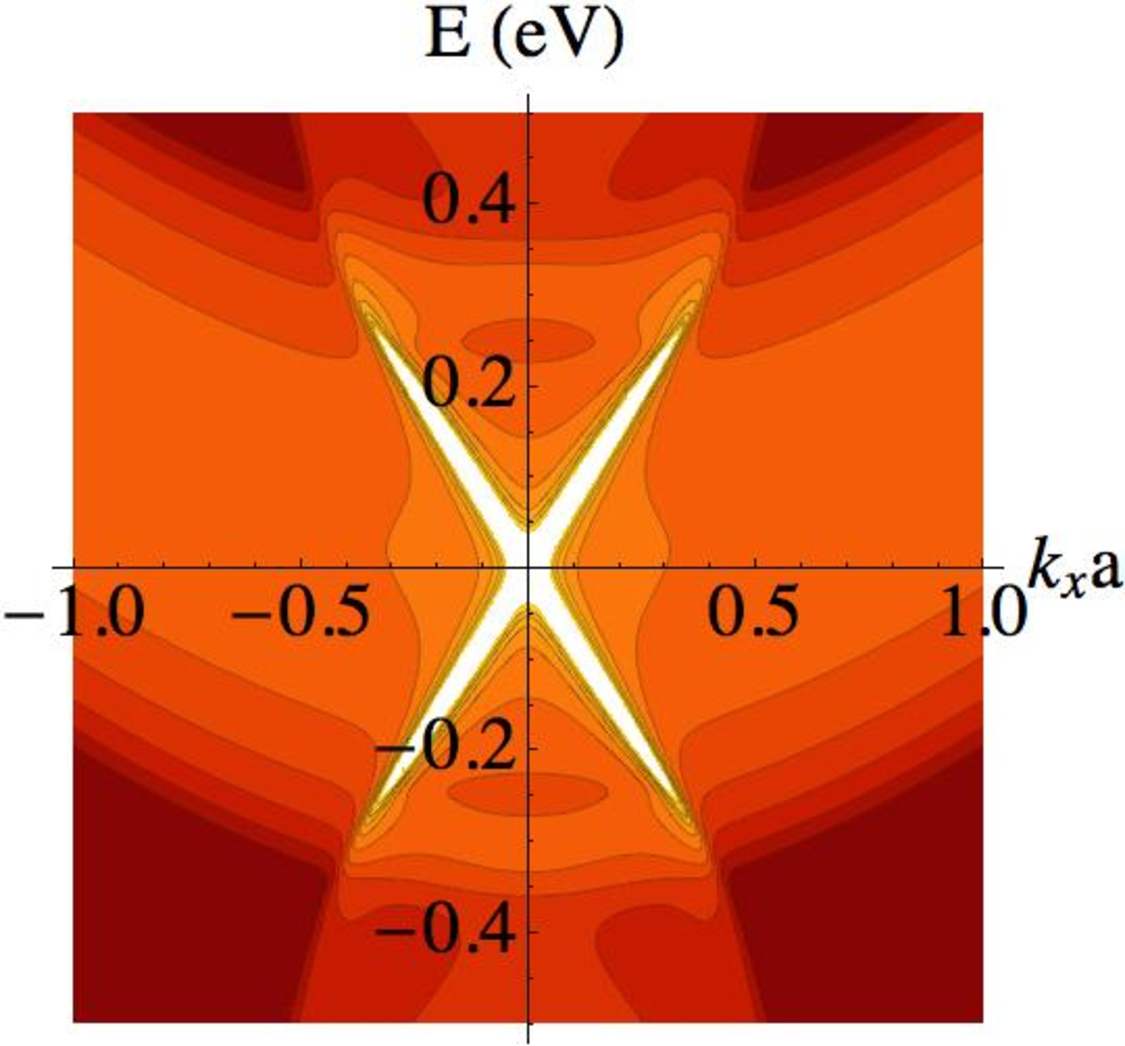
\includegraphics[width=1.7in]{j2.pdf}
\caption{The spectral function $N(E,k_x,k_y=0)$ at the interface of metal and topological insulator. Left: 
good contact, $J=t_M$, showing the continuum of metal induced gap states. 
Right: poor contact with low transparency, $J=0.2t_M$, showing well 
defined Dirac spectrum as on the TI surface. $t_M=0.18eV$, $\mu_M=-4t_M$, $a$ is lattice spacing.}
\end{figure}
%%%%%%%%%%%%%%%%%%%%%%%%%%
 
As a generic model for metal, we consider a single band tight binding Hamiltonian on cubic lattice,
\[
\mathscr{H}_L=\sum_{\kp,n,\sigma}[h({\kp})  n_{\kp,n,\sigma}
- t_M \phi_{\kp,n,\sigma}^\dagger  \phi_{\kp,n+1,\sigma} + h.c.] 
\]
where $h(\kp)=-2t_M(\cos k_x+\cos k_y)-\mu_M$. 
The Fermi surface parameters of the metal can be varied by tuning $t_M$ and $\mu_M$.
The metal occupies the left half space, $n\leq 0$, and 
the TI occupies the right half space $n\geq 1$. The interface domain consists of layer $n=0,1$. 
The coupling between metal and TI is described by hopping,
\[
\mathscr{H}_{LR}=-\sum_{\kp,\ell,\sigma}J_{\ell}\psi^{\dagger}_{\kp,n=1,\ell,\sigma}\phi_{\kp,n=0,\sigma}+h.c.
\]
$J_{\ell}$ is the overlap integral between the $p$-orbital $\ell=\pm$ of TI and the $s$-like orbital of metal. For simplicity, we assume $J_{\ell}$ is independent of spin. Then, $J_{+}=-J_{-}=J$. $J$ can be tuned from weak to strong. Small $J$ mimics a large tunneling barrier between M and TI, 
and large $J$ (comparable to $t_M$ or $B_2$) describes a good contact. 

%%%%%%%%%%%%%%%%%%%%%%%%%%
\begin{figure}
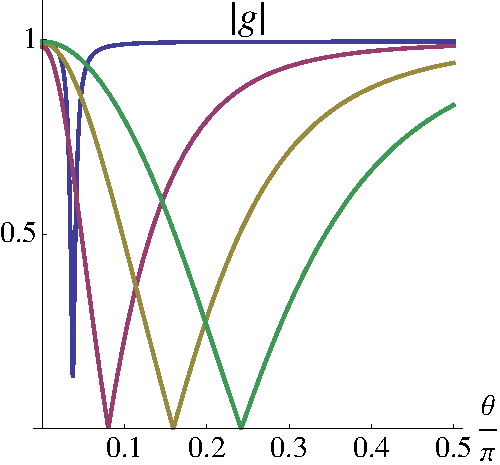
\includegraphics[width=1.7in]{la1.pdf}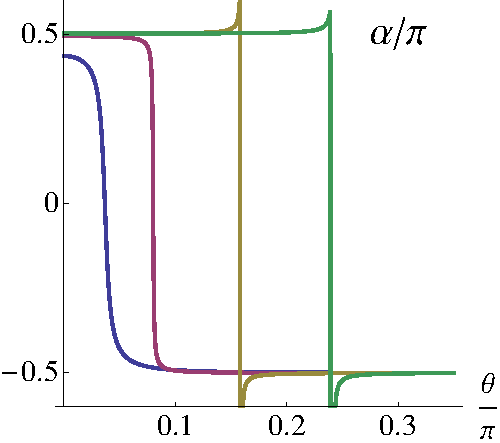
\includegraphics[width=1.7in]{la2.pdf}
\caption{The spin-conserving reflection amplitude $|g|$ and spin rotation angle 
$\alpha$ versus the incident angle $\theta$ for increasing contact transparency,
$J/t_M=0.25, 1, 1.5, 2$ (from left to right). $t_M=0.18eV$, $\mu_M=-4t_M$, $E=0.05$eV, $k_y=0$.
$|f|^2=1-|g|^2$. 
}
\end{figure}
%%%%%%%%%%%%%%%%%%%%%%%%%%

The lattice Green function of the composite system is computed via 
standard procedure by introducing the inter-layer transfer matrix 
and the method of interface Green function matching \cite{gf}. 
Fig. 4 shows two examples of the local spectral function 
(momentum-resolved density of states) at the interface,
\[ 
N(E,\kp)=-\sum_{n=0,1}\mathrm{Im Tr}\hat{\mathscr{G}}(E,\kp)_{n,n}, 
\]
where $\hat{\mathscr{G}}(E,\kp)_{n,n'}$ is 
the local Green function at the interface with $n,n'=0,1$, and  
the trace is over the spin and orbital space. 
In the tunneling (weak coupling, small $J$) limit, the interface spectrum includes 
a sharply defined Dirac cone as on the surface of TI. As $J$ is increased, 
the linearly dispersing mode becomes ill defined and eventually replaced 
by a continuum of metal induced gap states.

Once the lattice Green function is known for given incident $E$ and $k_{\parallel}$, 
the scattering (reflection) matrix can be constructed from $\hat{\mathscr{G}}$ by \cite{gf},
\[
\hat{S}(E,\kp)=\hat{\mathscr{G}}(E,\kp)_{0,0}g_M^{-1}(E,\kp)-\hat{1}
\]
where $g_M$ is the spin-degenerate bulk Green function of metal. Fig. 5 shows
the evolution of $|g(\theta)|$ and $\alpha(\theta)$ for increasing $J$, where 
a level broadening of $E/10$ is used. Most importantly,
we observe that the existence of a critical angel $\theta_c$, 
where complete spin-flip occurs and $\alpha$ jumps by $\pi$, is a robust phenomenon. 
It is independent of the details of the contact, the metal Fermi 
surface, or other high energy features in the band structure.

To understand the perfect spin flip, we first focus on 
the tunneling limit, $J\ll t_M$. In this limit, the local spectrum at layer $n=1$ as shown
in the right panel of Fig. 4 approaches
the TI surface spectrum, namely the helical Dirac cone. An incident up spin 
tunneling across the barrier will develop resonance with the helical mode, which is
a quasi-stationary state with long life time, if its 
momentum and energy satisfy $k_\parallel=E/A_2$. Moreover, it has to flip its spin, since 
only down spin can propagate in the $k_x$ direction (suppose $k_y=0$). 
The $\pi$ jump in the phase shift is also characteristic of the resonance. Indeed,
we have checked that precisely at $\theta_c$ the resonance criterion, $k_f\sin\theta_c=E/A_2$, 
is met.
We also varied $\mu_M$ for fixed $J$ and $t_M$, bigger $\mu_M$ 
yields a bigger Fermi surface and a smaller $\theta_c$. This is consistent with 
the resonance criterion above.

As $J$ is increased, the width of the resonance grows and eventually it is replaced by a 
broad peak (dip) in $|f|$ ($|g|$), but the vanishing of $|g|$ and $\pi$
shift in $\alpha$ at $\theta_c$ persist to good contacts,
even though in this limit the interface is flooded by MIGS (left panel of Fig. 4) 
and bears little resemblance to the Dirac spectrum.
With all other parameters held fixed, $\theta_c$ increases with $J$. Qualitatively,
coupling to TI renormalizes the metal spectrum near the interface, producing a smaller effective $k_f$ (hence a larger $\theta_c$) compared to its bulk value. 
It is remarkable that perfect spin flip at the critical angle persists all
the way from poor to good contacts. Indeed, the main features observed here for
for good contacts using the lattice model 
agree well with the results obtained in previous section by wave function matching. 

\section{Discussions}

We now discuss the experimental implications of our results. The M-TI interface spectrum can be measured by 
ARPES (or scanning tunneling microscope) experiments on metal film coated on a topological insulator.
Our results also suggest that a topological insulator can serve as a perfect mirror to flip the 
electron spin in metal. Such spin-active scattering at the M-TI interface may be 
exploited to make novel spintronic devices. The magnitude of $g$ or $f$
can be measured by attaching two ferromagnetic leads to a piece of metal in contact with TI, 
forming a multi-terminal device. 
One of the ferromagnetic leads produces spin-polarized electrons incident on the M-TI interface at some angle, while 
the other lead detects the polarization of reflected electron, as in a
giant magneto-resistance junction. The spin rotation angle $\alpha$ can be measured 
indirectly by comparing the predicted current-voltage characteristics of M-TI-M 
or Superconducto-TI-Superconductor junctions, which are sensitive the phase shift $\alpha$. It can also be inferred from 
the spin transport in a TI-M-TI sandwich, as discussed for QSH insulator in Ref. \cite{yokoyama09}.
Detailed calculations of the transport properties of these structured,
using the scattering matrix obtained here, will be subjects of future work.

\chapter{Superconducting Proximity Effect}

We present microscopic, self-consistent calculations of the 
superconducting order parameter and pairing correlations near the 
interface of an $s$-wave superconductor and
a three-dimensional topological insulator with spin-orbit coupling.
%
We discuss the suppression of the order parameter by the topological 
insulator and show that the equal-time pair correlation functions
in the triplet channel, induced by spin-flip scattering at the interface, 
are of $p_x\pm i p_y$ symmetry.
%
We verify that the spectrum at sub-gap energies is well described by
the Fu-Kane model. The sub-gap modes are viewed as interface states with
spectral weight penetrating well into the superconductor. 
We extract the phenomenological 
parameters of the Fu-Kane model from microscopic calculations, and find they
are strongly renormalized from the bulk material parameters. This is consistent 
with previous results of Stanescu et al for a lattice model using perturbation
theory in the tunneling limit.
\section{Introduction}
Fu and Kane showed that 
at the interface between a three-dimensional topological band insulator  (TI) and an 
$s$-wave superconductor (S) forms a remarkable two-dimensional non-Abelian superconductor \cite{f-k}.
It hosts Majorana zero modes at vortex cores, as in a 
$p_x+ip_y$ superconductor \cite{r-g}, but respects time-reversal symmetry. 
As argued in Ref. \cite{f-k}, the presence of superconductor induces a pairing interaction
between the helical Dirac fermions at the surface of the topological insulator,
and gaps out the surface spectrum. Then, the interface can be modeled elegantly by 
 a simple matrix Hamiltonian in Nambu space (we follow the convention of Ref. \cite{qi-zhang}),
\begin{equation}
H_{FK}(\mathbf{k})=\left(
\begin{array}{cc}
h_s(\mathbf{k})  &  i\sigma_y  \Delta_s \\
-i\sigma_y \Delta_s^*  &   -h_s^*(-\mathbf{k})
\end{array}\label{fkmodel}
\right),
\end{equation}
where $\mathbf{k}=(k_x,k_y)$ is the two-dimensional momentum in
the interface plane, $\sigma_i$ are the Pauli matrices,
$h_s(\mathbf{k})$ is the surface Hamiltonian
for the topological insulator describing the helical Dirac fermions \cite{qi-zhang,rmp},
\begin{equation}
h_s(\mathbf{k})=-\mu_s + v_s (\sigma_xk_y-\sigma_y k_x).
\end{equation}
Fu and Kane also proposed to use S-TI proximity structures to
generate and manipulate Majorana fermions which obey non-Abelian 
statistics and are potentially useful for fault tolerant quantum 
computation \cite{f-k}. 
This proposal and a few others that followed based on 
superconductor-semiconductor heterostructures \cite{roman,maryland,jason,mao1,mao2} have revived
the interest in superconducting proximity effect involving insulating/semiconducting 
materials with spin-orbit coupling. More complex S-TI proximity structures
with ferromagnets \cite{yu,jacF} or unconventional superconductors \cite{jacU} 
have been investigated.

Experiments are beginning to realize various S-TI proximity structures \cite{sca,march}.
In light of these developments, it is desirable to
understand to what extent the effective model $H_{FK}$ holds,
and what are the values of $(\Delta_s,\mu_s,v_s)$ for given materials. 
Answering these questions is crucial for future experiments designed to probe
and manipulate Majorana fermions. As a first step in this
direction, Stanescu et al considered a microscopic lattice model
for the TI-S interface \cite{stan}. In this model, TI and S are described by a tight binding 
Hamiltonian defined on the diamond and hexagonal lattice respectively.
The two materials are coupled by tunneling term in the Hamiltonian. 
These authors found that 
for small $\mathbf{k}$, $H_{FK}(\mathbf{k})$ is valid but its parameters are 
significantly renormalized by the presence of the superconductor. 
This is supported by leading order 
perturbation theory in the weak coupling (tunneling) limit. They also
discussed the induced $p$-wave correlation within the framework of
perturbation theory. The $p$-wave correlation has also been noted in 
an analogous proximity structure in two dimension between
a quantum spin Hall insulator and a superconductor \cite{ann}.


In this work, we consider S-TI proximity structures where 
S and TI are {\it strongly} coupled to each other, 
rather than being separated by a tunneling barrier.
This is the desired, presumably the optimal, configuration to realize the Fu-Kane
proposal, e.g. to achieve maximum value of $\Delta_s$ in $H_{FK}$ for given
superconductor. 
In the strong coupling limit, 
the modification of superconductivity by the TI becomes important.
This includes the suppression of the superconducting order parameter,
the induction of triplet pair correlations by spin-active scattering
at the interface, and the formation of interface states below the bulk superconducting gap.
In order to accurately answer questions raised in the preceding paragraph
for strongly coupled S-TI structures, one has to self-consistently 
determine the the spatial profile of 
the order parameter near the interface.

Our work is also motivated by recent experimental discovery that Copper-doped 
topological insulator Cu$_x$Bi$_2$Se$_3$
becomes superconducting at a few Kelvins \cite{cu1,cu2,ando}. It 
seems possible then to combine such superconductors with topological insulator 
Bi$_2$Se$_3$ to achieve strong proximity coupling. 
% Using Bi$_2$Se$_3$ and Cu$_x$Bi$_2$Se$_3$ as one of the examples,
We set up microscopic, continuum models for the S-TI structures and solve the result 
Bogoliubov-de Gennes (BdG) equation numerically.
We first compute the superconducting order 
parameter as a function of the distance
away from the interface.
We then verify the validity of the Fu-Kane effective model
and extract its parameters from the low energy sector of the energy
spectrum. The emergence
of $H_{FK}$ will be viewed as the result of the ``inverse proximity effect", namely
strong modification of superconductivity by the presence of TI.
This is in contrast to the previous viewpoint of
pairing between surface Dirac fermions, which is a more proper description
in the tunneling limit.
The spectral weight of these low energy modes (with energy below the bulk superconducting gap) 
are shown explicitly to peak near the interface but penetrate well
into the superconductor.
We will also show analytically that the induced triplet pair
correlations are of $p_x\pm ip_y$ orbital symmetry, and systematically
study their spatial and momentum dependence.
Our results connect the phenomenological theory of Fu and Kane \cite{f-k}
to real materials. Our results for continuum models and strong coupling 
limit are also complementary to the results of Stanescu et al \cite{stan}
for lattice models and tunneling limit.

In what follows, we first outline the formulation of the problem and 
then present the main results. Technical details on numerically solving
the BdG equation are relegated to the appendix.

\section{Model and Basic Equations}

The band gaps of topological insulators are much larger than the superconducting
gap of all  weak coupling $s$-wave superconductors. 
For the purpose of studying the proximity
effect between such superconductors and topological insulators, it is
sufficient to describe the topological insulator using the 
low energy effective $\mathbf{k}\cdot \mathbf{p}$ Hamiltonian. Following
Zhang et al \cite{zhang}, we model Bi$_2$Se$_3$ by 
\begin{eqnarray}
H_{TI}({\bf k})=
\left( \begin{array}{cccc}
M({\bf k}) & 0 & A_1 k_z  & A_2 k_{-} \\
0 &M({\bf k})& A_2 k_+ & -A_1 k_z \\
 A_1 k_z  & A_2 k_{-} &-M({\bf k}) & 0 \\
A_2 k_+ & -A_1 k_z &0 & -M({\bf k}) \\
 \end{array} \right)-\mu \hat{I}.
 \end{eqnarray}
Here $k_{\pm}=k_x \pm i k_y $, 
$M({\bf k})=M-B_1 k_z ^2 - B_2 (k_x^2 + k_y^2)$, and $\hat{I}$ is $4\times 4$
unit matrix. The numerical values of 
the parameters are obtained from first principle calculations \cite{zhang,band}, $M=0.28$ eV,
$A_1=2.2$ eV\AA, $A_2=4.1$ eV\AA, $B_1=10$ eV\AA$^2$, $B_2=56.6 $ eV\AA$^2$.
We work in basis $\{\ket{1\uparrow}, \ket{1\downarrow},\ket{2\uparrow},\ket{2\downarrow} \}$,
where 1 (2) labels the $P1_z^+$ ($P2_z^+$) orbital \cite{zhang}. Note that
we have neglected the unimportant diagonal term $\epsilon_0({\bf k})$ in Ref. \cite{zhang} which 
only slightly modifies the overall curvature of the band dispersion. We also
keep the chemical potential $\mu$ as a tuning parameter.

We consider a simple model of superconductor derived from a metallic
state obtained by turning off the spin-orbit coupling ($A_1=A_2=0$) in
$H_{TI}$ and tuning the Fermi level well into the conduction band \cite{zhao}. The metal
Hamiltonian
\begin{eqnarray}
H_{M}({\bf k})=\mathrm{diag} [M({\bf k}), M({\bf k}), -M({\bf k}), -M({\bf k})]-E_f \hat{I},
\end{eqnarray}
with  $E_f>M$. 
This mimics electron-doping the topological insulator \cite{cu2} 
or equivalently electrochemically
shifting its chemical potential by applying a gate voltage \cite{gate}.
As shown in Fig. \ref{setup}, 
the valence band (band 1 with dispersion $M({\bf k})-E_f$) is well below the Fermi level and remains inert as far as 
superconductivity is concerned.  Next, within the framework of Bardeen-Cooper-Schrieffer
theory, we assume attractive interaction between
the electrons in the conduction band (band 2) near the Fermi surface described by the reduced
 Hamiltonian,
\begin{equation}
H_{int}=\sum_{\bf k} \psi^\dagger_{2\uparrow}({\bf k})\psi^\dagger_{2\downarrow}(-{\bf k})\Delta + h.c.
\end{equation}
Here $\Delta$ is the 
superconducting order parameter, $\psi^\dagger_{l\sigma}$ is the electron creation operator for orbital $\l=1,2$ and
spin $\sigma=\uparrow,\downarrow$. The superconductor is then described by 
\begin{equation}
H_S=\sum_{{\bf k},l,\sigma}\psi^\dagger_{l\sigma}({\bf k})H_M({\bf k})_{l\sigma,l\sigma}\psi_{l\sigma}({\bf k})+H_{int}.
\end{equation}
Note that $H_S$ and $H_{TI}$ are in the same 
basis.

This model can serve as a generic model for $s$-wave superconductors with negligible
spin-orbital coupling. Whether it can actually describe the superconductor Cu$_x$Bi$_2$Se$_3$
has to be settled by future experiments.
The transition temperature of Cu$_x$Bi$_2$Se$_3$ 
at optimal doping $x=0.12$ is $T_c=3.8$K, which corresponds to a zero 
temperature superconducting gap $\Delta\sim$0.6meV \cite{cu1,cu2,ando}. The Fermi level is 0.25eV 
above the bottom of the conduction band, and the Fermi wave vector $k_f\sim 0.12$\AA$^{-1}$.
The pairing symmetry of Cu$_x$Bi$_2$Se$_3$ is to our best knowledge is unknown at present (it appears
to be fully gapped from the specific heat measurement \cite{ando} and might be a 
topological superconductor \cite{cu2}). 
If it turns out to be a conventional $s$-wave superconductor, its mains 
features will be captured by $H_S$ above with suitable choice of $E_f$ and $\Delta$.

%%%%%%%%%%%%%%%%%%%%%%%%%%
\begin{figure}
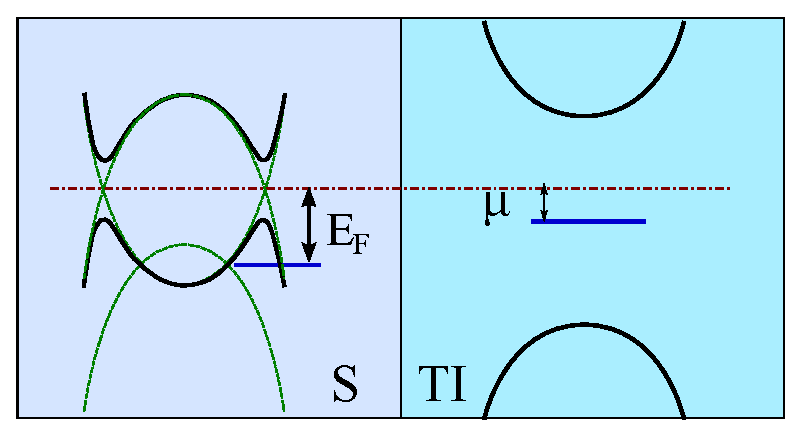
\includegraphics[width=3in]{setup.eps}
\caption{Schematic (not to scale) band diagrams  in a superconductor-topological insulator (S-TI) proximity
structure. $E_f$ is the Fermi energy of the metal described by $H_M$ measured from the band crossing point. $\mu$ is
the chemical potential of TI measured from the band gap center. The superconducting gap
is much smaller than the band gap of TI.
}\label{setup}
\end{figure}
%%%%%%%%%%%%%%%%%%%%%%%%%%

Now consider a proximity structure consisting 
of a superconductor at $z<d$ and a topological insulator at $z>d$ (Fig. \ref{setup}).
The interface at $z=d$ is assumed to be specular, so the momentum $\mathbf{k_\parallel}=(k_x,k_y)$ 
parallel to the interface is conserved. The Hamiltonian for the whole system 
\begin{align}
\mathcal{H} = &\int d \mathbf{k}_\parallel dz
\Bigl\{ \sum_{\sigma} \psi^{\dagger}_{1 \sigma}(\mathbf{k}_\parallel,z)[h_0 - \mu(z)] \psi^{\dagger}_{1 \sigma}(\mathbf{k}_\parallel,z) 
 \nonumber \\
&- \sum_{\sigma} \psi^{\dagger}_{2 \sigma}(\mathbf{k}_\parallel,z)[h_0 + \mu(z)] \psi^{\dagger}_{2 \sigma}(\mathbf{k}_\parallel,z)\nonumber \\
&+\Delta(z)  \psi^{\dagger}_{2 \uparrow}(\mathbf{k}_\parallel,z) \psi^{\dagger}_{2 \downarrow} (-\mathbf{k}_\parallel,z)+h.c.\nonumber \\
&+A_1(z) [\psi^{\dagger}_{1 \uparrow} (-\idz) \psi_{2 \uparrow} 
+\psi^{\dagger}_{1 \downarrow} (\idz) \psi_{2 \downarrow}+h.c.]  \nonumber\\
&+A_2(z)
[\psi^{\dagger}_{1 \uparrow} \ki \psi_{2 \downarrow} +\psi^{\dagger}_{1 \downarrow} \kp \psi_{2 \uparrow} +h.c.]
\Bigr \}. \label{hbH}
\end{align}
Here $h_0(\mathbf{k}_\parallel, \partial_z)=M -B_1 \partial_z^2 -B_2 k_\parallel^2$, $\mu(z)$ and $A_i(z)$
are piece-wise constant, 
\begin{align}
\mu(z)&=E_f\theta(d-z)+\mu\theta(z-d),\\
A_i(z)&=A_i\theta(z-d),\;\;i=1,2
\end{align}
in terms of the step function $\theta$. The order parameter obeys the gap equation
\begin{equation}
\Delta(z) = g(z) \int d \mathbf{k}_\parallel \langle {\psi_{2 \uparrow}(\mathbf{k}_\parallel,z) \psi_{2 \downarrow}(-\mathbf{k}_\parallel,z) }\rangle. \label{gapE}
\end{equation}
We assume $g(z)=g\theta(d-z)$, the coupling constant $g$ determines the bulk gap.

To self-consistently solve Eq. \eqref{hbH} and \eqref{gapE}, we introduce
Bogoliubov transformation
\begin{equation}
 \psi_{l \sigma}(\mathbf{k}_\parallel,z) = \sum_n  u_{n,l \sigma} (\kperp, z) \gamma_{n,\kperp} + v^\ast_{n,l \sigma} (\kperp, z) \gamma_{n,\kperp}^\dagger
\end{equation}
to diagonalize $\mathcal{H}$ as
\begin{equation}
\mathcal{H} = E_g + \int d \kperp\sum_n \epsilon_n(k_\parallel) \gamma_{n,\kperp}^\dagger \gamma_{n,\kperp} ,
\end{equation}
where $E_g$ is the ground state energy, and $\gamma_{n,\kperp}^\dagger$
is the creation operator of Bogoliubov quasiparticles with energy $\epsilon_n(k_\parallel)$.
The wave function $u$ and $v$ satisfy the following Bogliubov-de Gennes (BdG) equation,
\begin{equation}
\hat{H}_{B}(\mathbf{k}_\parallel,z) \hat{\phi}_n(\mathbf{k}_\parallel,z)=\epsilon_n(k_\parallel)\hat{\phi}_n (\mathbf{k}_\parallel,z).
\label{bdgsimp}
\end{equation}
Here, the BdG Hamiltonian
\begin{equation}
\hat{H}_{B}=\left( \begin{array}{cccc}
h_0 -\mu  & \mathbf{d} \cdot \boldsymbol{\sigma}&0&0\\ 
 \mathbf{d} \cdot \boldsymbol{\sigma} &-h_0 -\mu &0&-\Delta\, i\sigma_y\\ 
0 &0& \mu -h_0 & \mathbf{d} \cdot \boldsymbol{\sigma}^* \\
0 &\Delta^{\ast} \, i\sigma_y & \mathbf{d} \cdot \boldsymbol{\sigma}^* & \mu+h_0\\ 
 \end{array} \right), \label{bdgH} 
\end{equation}
and the wave function (dropping the arguments)
\begin{equation}
\hat{\phi}_n=(u_{n,1\uparrow}, u_{n,1\downarrow}, u_{n,2\uparrow}, u_{n,2\downarrow}, 
v_{n,1\uparrow}, v_{n,1\downarrow}, v_{n,2\uparrow}, v_{n,2\downarrow})^\mathrm{T}.
\end{equation}
The vector $\mathbf{d}(\mathbf{k}_\parallel,z)$ is defined as
\begin{equation}
d_x=A_1(z)k_x,\,\, d_y=A_1(z)k_y,\,\, d_z=A_2(z)(-i\partial_z).
\end{equation} 
Other quantities such as $h_0(\mathbf{k}_\parallel,z)$, $\mu(z)$, and $\Delta(z)$ are 
defined above.
In terms of the wave functions, the zero temperature gap equation becomes
\begin{equation}
\Delta(z) = g(z) \int d \mathbf{k}_\parallel \sum_n' u_{n,2 \uparrow}(\mathbf{k}_\parallel,z) v^*_{n,2\downarrow}(-\mathbf{k}_\parallel,z) ,
\end{equation}
where the summation denoted by prime is restricted to $0<\epsilon_n<\omega_D$ with 
$\omega_D$ being the Debye frequency.


We will exploit a particular symmetry of the BdG Hamiltonian to simplify 
calculations. Define the polar angle $\varphi_k$ for the in-plane wave vector $\kperp$, 
\begin{equation}
k_x+ik_y=k_{\parallel}e^{i\varphi_k}.
\end{equation}
Then the BdG Hamiltonian for arbitrary $(k_x,k_y)$ is
related to that for $(k_x=k_\parallel,k_y=0)$ by unitary transformation 
\begin{equation}
\hat{U}^\dagger(\kperp) \hat{H}_{B}(k_x,k_y) \hat{U}(\kperp) = \hat{H}_{B}(k_\parallel,0).
\label{symm}
\end{equation}
Here $U$ is a 
block diagonal matrix,
\begin{equation}
U(\kperp)=\mathrm{diag}[e^{-i\sigma_z\frac{\varphi_k}{2}}, e^{-i\sigma_z\frac{\varphi_k}{2}}, e^{i\sigma_z\frac{\varphi_k}{2}},e^{i\sigma_z\frac{\varphi_k}{2}} ]. \label{unit}
\end{equation}
Thus, the eigen energy $\epsilon_n$ only depends on the magnitude of $\kperp$.
Once the wave function for $\varphi_k=0$ is known, the wave function for $\varphi_k\in (0,2\pi)$
can be obtained by simple unitary transformation.

We solve the matrix differential equation \eqref{bdgsimp} by conserving it into an algebraic equation, 
following the treatment of superconductor-ferromagnet structure by 
Halterman and Valls \cite{h-v}. The whole S-TI proximity structure is assumed to have 
finite dimension $L$ in the $z$
direction. The superconductor occupies the region $0<z<d$,
while the topological insulator occupies $d<z<L$. Hard wall boundary conditions are enforced at the end points, 
$z=0$ and $z=L$.  
The exact boundary conditions at the end points only affect the local physics there, provided 
that the boundaries are sufficiently far away from the S-TI interface. We expand the wave function
and order parameter in Fourier series \cite{h-v},
\begin{align}
u_{n,l\sigma}(z) &= \sum_m u_{nm}^{l \sigma}\,\phi_m(z),\label{uexp}\\ 
v_{n,l\sigma}(z) &= \sum_m v_{nm}^{l \sigma}\, \phi_m(z),\\
\quad \Delta(z) &= \sum_m \Delta_{m}\, \phi_m(z) , \label{Dexp}\\
\phi_m(z)&=\sqrt{2/L}\sin(k_m z).
\end{align}
The integer $m=1,2,...,N$ labels the quantized longitudinal (along $z$) momentum $k_m=m\pi/L$. 
The cutoff $N$ is chosen as \cite{s-v}
\begin{equation}
B_1k^2_N=M+E_f+\omega_D. \label{eq-N}
\end{equation}
By expansion Eq. \eqref{uexp}-\eqref{Dexp}, the BdG equation
becomes an $8N \times 8N$ matrix equation. With a reasonable guess of the order parameter profile, 
the eigen energies and eigen wave functions are obtained by solving the matrix eigen value problem.
Then a new order parameter profile is computed from the gap equation. The procedure is iterated
until convergence is achieved.  Relevant technical details can be found
in the Fourier calculations section. 

To analyze the spectrum of the system, it is convenient to define the retarded Green's function
\begin{equation}
G^R_{l\sigma}(\mathbf{k}_\parallel,z,t)=-i\theta(t)\langle \{\psi_{l\sigma}(\mathbf{k}_\parallel,z,t),
\psi^\dagger_{l\sigma}(\mathbf{k}_\parallel,z,0)\}\rangle
\end{equation}
where the time-dependent field operators are in Heisenberg picture. 
For given $\kperp$ and $z$, the spectral functions 
are defined as
\begin{align}
&N_{l\sigma}(\mathbf{k}_\parallel,z,\omega)= -\mathrm{Im}G^R_{l\sigma}(\mathbf{k}_\parallel,z,\omega), \\
&N(\mathbf{k}_\parallel,z,\omega)=\sum_{l\sigma}N_{l\sigma}(\mathbf{k}_\parallel,z,\omega).
\end{align}
In terms of the wave functions and eigen energies, 
\begin{equation}
N_{l\sigma}(\mathbf{k}_\parallel,z,\omega>0)=\sum_n|u_{n,l\sigma}(\mathbf{k}_\parallel,z)|^2\delta(\omega-\epsilon_n). 
\end{equation}
We also introduce the equal-time pair correlation functions
for the conduction electrons 
\begin{equation}
F_{\alpha\beta}(\mathbf{k}_\parallel,z)=\langle \psi_{2\alpha}(\mathbf{k}_\parallel,z) \psi_{2\beta}(-\mathbf{k}_\parallel,z)\rangle.\label{pair-corr}
\end{equation}
For example, at zero temperature we have
\begin{align}
F_{\uparrow\uparrow}(\mathbf{k}_\parallel,z)=\sum'_n u_{n,2\uparrow}(\mathbf{k}_\parallel,z)
v^*_{n,2\uparrow}(-\mathbf{k}_\parallel,z),\\
F_{\downarrow\downarrow}(\mathbf{k}_\parallel,z)=\sum'_n u_{n,2\downarrow}(\mathbf{k}_\parallel,z)
v^*_{n,2\downarrow}(-\mathbf{k}_\parallel,z).
\end{align}
Triplet components of $F$ will be induced near the S-TI interface by spin-active
scattering \cite{zhao}.

%\appendix*
\section{Fourier Calculations}
We follow the numerical scheme of Halterman and Valls to solve 
the matrix BdG equation \cite{h-v}. The wave functions and the order parameter
are expanded in the orthonormal basis $\{\phi_m(z)\}$, with $m=1,...,N$. For example,
function $u_{n,1\uparrow}(z)$ is represented by $N$ numbers,
\begin{align*}
(u^{1\uparrow}_{n,1},u^{1\uparrow}_{n,2},...u^{1\uparrow}_{n,m}...,u^{1\uparrow}_{n,N}).
\end{align*}
Accordingly, each term in $\hat{H}_{B}$ is represented
by a $N\times N$ matrix with the matrix elements given by
\begin{align*}
h_0(\kperp,\partial_z) &\rightarrow \delta_{mm'}(M - B_1 k_m^2 - B_2 k_\parallel^2) \\
U(z) &\rightarrow E_f E_{mm'} + \mu F_{mm'} \\
 A_2(z) \partial_z &\rightarrow A_2 G_{mm'}\\
 A_1(z) k_\pm &\rightarrow A_z k_\pm F_{mm'} \\
 \Delta &\rightarrow D_{mm'}\equiv \sum_{m''}J_{m,m',m''}\Delta_{m''}
\end{align*}
where 
\begin{align*}
E_{mm'}&=\int_0^{d} \phi_m(z) \, \phi_{m'}(z) dz \\
F_{mm'}&=\int_d^{L} \phi_m(z) \, \phi_{m'}(z) dz \\
G_{mm'}&=\int_d^{L} \phi_m(z) \partial_z \phi_{m'}(z) dz\\
J_{m,m',m''}&=\int_0^{d} \phi_m(z) \, \phi_{m'}(z) \, \phi_{m''}(z) dz
\end{align*}
These integrals can be evaluated analytically. Then the BdG equation becomes
an $8N\times 8N$ matrix equation. The gap equation can be rewritten as
\[
\Delta_{m}=g\int d\kperp \sum'_n \sum_{m',m''} J_{m,m',m''}
u^{2\uparrow}_{nm'}(\kperp)v^{2\downarrow}_{nm''}(-\kperp)^* 
\]
The integral over $\kperp$ is first simplified to an integral over $k_\parallel$
by the symmetry Eq. \eqref{symm} and then evaluated numerically with high 
momentum cutoff 
$\sqrt{(E_F+\omega_D+M)/B_2}$.


\section{The Order Parameter}

%%%%%%%%%%%%%%%%%%%%%%%%%%
\begin{figure}
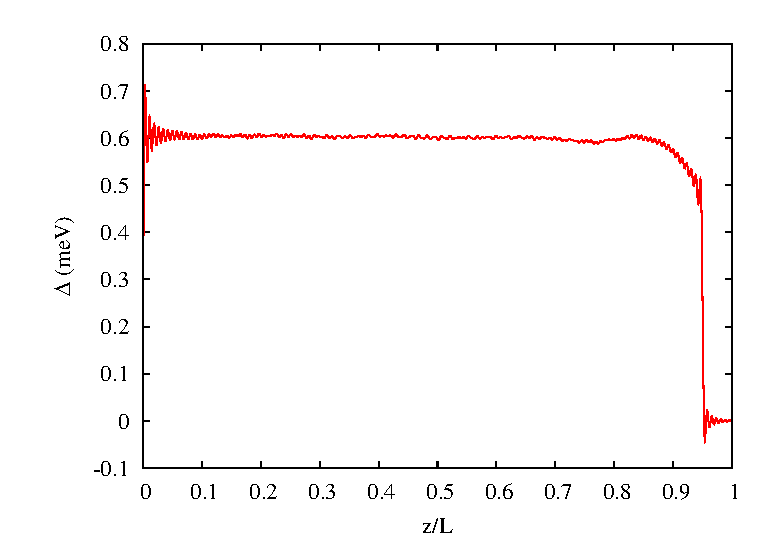
\includegraphics[width=3.4in]{delta-cu.eps}
\caption{The superconducting order parameter $\Delta(z)$ near an S-TI interface at $
z=d=0.95L$. The superconductor occupies $0<z<d$, and topological insulator occupies $d<z<L$. 
$L=300$ nm, $\mu$=0, the bulk gap $\Delta_0=$0.6meV. }\label{delta-cu}
\end{figure}
%%%%%%%%%%%%%%%%%%%%%%%%%%

First we present the spatial profile of the superconducting order parameter $\Delta(z)$
after the convergence is achieved. In all following calculations, $E_f$ is fixed at 0.4eV, 
which is modeled after optimally doped Cu$_x$Bi$_2$Se$_3$ \cite{cu2}. And the Debye frequency
is set as $\omega_D=0.1E_f$ \cite{h-v}.
%
Fig. \ref{delta-cu} shows an example with $\mu=0$, $L=300$nm, $d=0.95L$, and
a bulk gap of 0.6meV as found in Cu$_x$Bi$_2$Se$_3$. 
%
Going from the superconductor into the topological insulator,
$\Delta$ first gets suppressed as the interface is approached before it
drops to zero inside TI. The suppression is roughly 20\% at the interface.
Note that the fine wiggles of $\Delta$ in the simulation results 
are due to the finite momentum cutoff of 
the longitudinal momentum $k_m$. As previously discussed by 
Stojkovic and Valls \cite{s-v}, the number of oscillations is $\sim N/2$, and the 
oscillation amplitude vanishes in the bulk as $N$ is increased. 
In this case, $N$ is chosen to be
258 according to Eq. \eqref{eq-N}. So the matrix to be diagonalized is 2064 by 2064.

Fig. \ref{delta-24} show the result for $\mu=0$, $d=0.9L$, and 
a superconductor with bulk gap $\Delta_0\sim 2.4$meV. Since the coherence length
is much smaller than the previous example, it is sufficient to consider 
$L=160$nm, and correspondingly $N=138$. 
The order parameter profile  
depends weakly on $\mu$, as shown in Fig. \ref{delta-chem} for a superconductor
with bulk gap $\sim 5.2$meV. 
From these examples, one observes that the length scale over which $\Delta$ is 
significantly suppressed does {\it not} scale with $\xi_0$, the zero temperature
coherence length of the superconductor. Rather it stays roughly the same, 
on the order of $30$nm, as $\xi_0$ is varied over one decade from Fig. \ref{delta-cu}
to Fig. \ref{delta-chem} (note the horizontal axis is $z/L$). 
This is not very surprising since $\xi_0$ is not the only length scale at play here.
The interface represents a strong (as compared to $\Delta_0$) perturbation that 
significantly distorts the bulk wave functions.
The self-consistent microscopic BdG approach provides a reliable way to
capture the details of $\Delta(z)$ near the interface.


%%%%%%%%%%%%%%%%%%%%%%%%%%
\begin{figure}
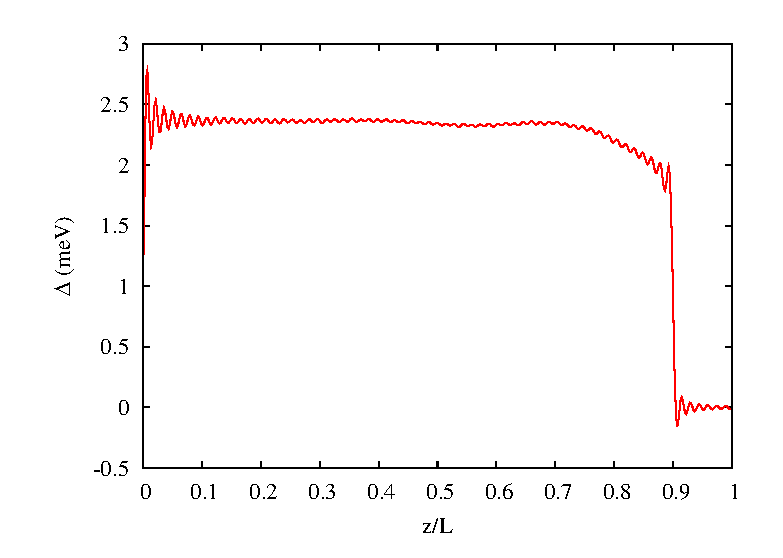
\includegraphics[width=3.4in]{dt.eps}
\caption{The order parameter $\Delta(z)$ near an S-TI interface at $
z=d=0.9L$. $L=160$ nm, $\mu$=0, $\Delta_0\sim 2.4$meV.}
\label{delta-24}
\end{figure}
%%%%%%%%%%%%%%%%%%%%%%%%%%


%%%%%%%%%%%%%%%%%%%%%%%%%%
\begin{figure}
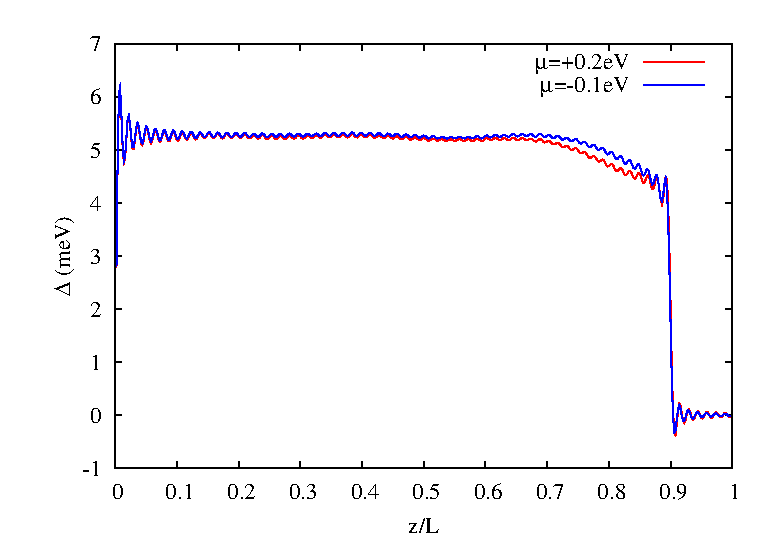
\includegraphics[width=3.4in]{dtchemi.eps}
\caption{The order parameter profile for two different chemical potentials of
the topological insulator, $\mu=-0.1$eV and $\mu=0.2$eV. $L=160$nm,  
$\Delta_0\sim 5.2$meV. }\label{delta-chem}
\end{figure}
%%%%%%%%%%%%%%%%%%%%%%%%%%

It is illuminating to compare the proximity effect in S-TI
structure with that in S-F structure \cite{toku}, where F stands for 
a ferromagnetic insulator. 
The presence of F breaks time-reversal and spin rotation symmetry and 
significantly suppresses the order parameter. The suppression is
sensitive to the spin mixing angle which is related to the band gap
and exchange field of F \cite{toku}.
In contrast, despite the spin-active scattering of electrons 
by TI which introduces spin-flips and spin-dependent phase shifts \cite{zhao}, 
spin-orbit coupling is not pair breaking.
%
The suppression of $\Delta$ near the interface is to a large extent 
due to the reorganization of local wave functions enforced by the boundary conditions 
at $z=d$ for piece-wise potentials $\mu(z)$, $A_i(z)$, $g(z)$. 
It depends on for example how the wave functions decay inside the TI
for given $E_f$ and $\mu$, and involves ``high-energy" physics beyond the
scale of $\Delta$ but below the scale of the band gap. 
%
To test this, we have investigated the proximity effect between the same
superconductor and
a hypothetical ordinary insulator modeled by $H_{TI}$ with $A_1=A_2=0$
and the same band gap. The suppression of $\Delta$ by such an 
ordinary insulator turns out to be very similar. 

\section{The Interface Mode and The Fu-Kane Model}

Next we analyze the energy spectrum of the system, $\epsilon_n(k_\parallel)$,
obtained from the BdG calculation. 
Take the case of $\mu=0$, $L=160$nm, $d=0.9L$, $\Delta_0\sim 5.2$meV as an example.
Fig. \ref{lev-fk} shows the first several energy levels of the composite
system versus the transverse momentum $k_\parallel$. There are many continuously
dispersing modes at energies above the bulk gap. They are the usual Bogoliubov
quasiparticles for different quantized longitudinal momenta.
One also sees a series of avoided level crossings.
At small $k_\parallel$ emerges a well-defined mode below $\Delta_0$. We will 
identify it as the interface mode first discussed by Fu and Kane \cite{f-k}.

The Fu-Kane model Eq. \eqref{fkmodel} predicts the dispersion 
\begin{equation}
E(k)=\sqrt{|\Delta_s|^2+(v_sk \pm\mu_s)^2}.
\end{equation}
We fit the very low energy portion of the spectrum to this prediction to
extract the phenomenological parameters in the Fu-Kane model. The result
is shown in Fig. \ref{lev-fk}. We find that,
not surprisingly, $\Delta_s=1.8$meV which is much smaller than $\Delta_0=5.2$meV, and 
$v_s=2.7$eV$\mathrm{\AA}$ which deviates significantly 
from $A_2=4.2$eV$\mathrm{\AA}$ predicted for the surface 
dispersion of TI. Moreover, $\mu_s=7.5$meV despite that the chemical potential
of TI is $\mu=0$. Therefore, our results show that the values of $(\Delta_s,v_s,\mu_s)$
are strongly renormalized by the presence of the superconductor. This is consistent 
with the findings of Stanescu et al for weakly coupled S-TI structures \cite{stan}. 

%%%%%%%%%%%%%%%%%%%%%%%%%%
\begin{figure}
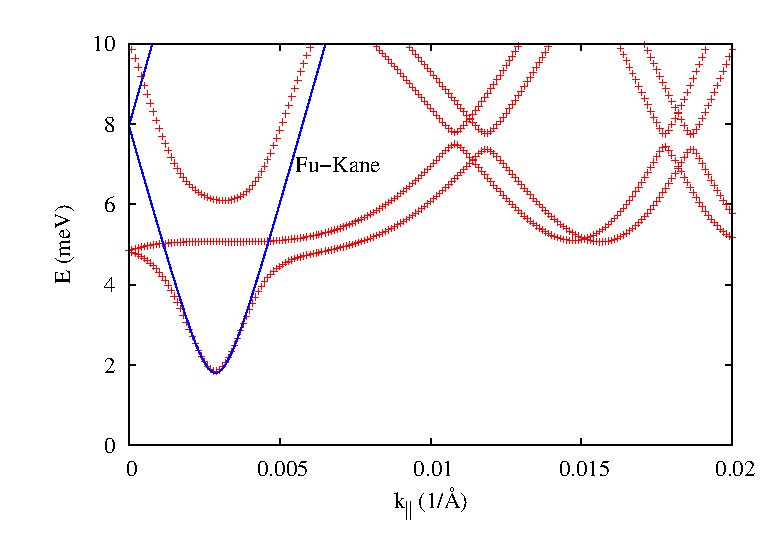
\includegraphics[width=3.4in]{levels.eps}
\caption{The lowest few energy levels $\epsilon_n(k_\parallel)$. 
$\mu=0$, $L=160$nm, and the bulk superconducting gap $\Delta_0\sim$5.2meV.
A well-defined interface mode is clearly visible at sub-gap energies.
Solid lines show a fit to the Fu-Kane model, with $\Delta_s=1.8$meV, 
$v_s=2.7$eV\AA, and $\mu_s=7.5$meV.
}\label{lev-fk}
\end{figure}
%%%%%%%%%%%%%%%%%%%%%%%%%%

We have checked the validity of the Fu-Kane model for a variety of chemical potentials.
Representative examples are plotted in Fig. \ref{lev-chem}. In each case, the sub-gap 
mode can be well accounted by the Fu-Kane 
model with suitable choice of parameters. While $\mu_s$ is always different from $\mu$,
numerically we find it scales linearly with $\mu$. At the same time, 
$\Delta_s$ and $v_s$ show no strong dependence on $\mu$ for this set of parameters.
To make sure that the sub-gap mode is indeed localized near the interface, we plot in 
Fig. \ref{sp} the $z$ dependence of the spectral function $N(k_\parallel,z,\omega)$.
%
The spectral weight of the sub-gap mode is peaked near the interface and decays over 
a length scale $\sim \xi_0$ into the superconductor. This result clearly shows
that for strongly coupled S-TI interfaces, the Fu-Kane model actually describe a
rather ``fat" interface mode. Note that the spectral weight on the TI side 
(not shown in the figure) is finite, 
but it is much smaller in magnitude and decays very fast inside TI. Finally,
Fig. \ref{dos} shows the local density of states near the interface.
The interface mode leads to finite density of states below the bulk gap,
but the spectral weight is very small.

%%%%%%%%%%%%%%%%%%%%%%%%%%
\begin{figure}
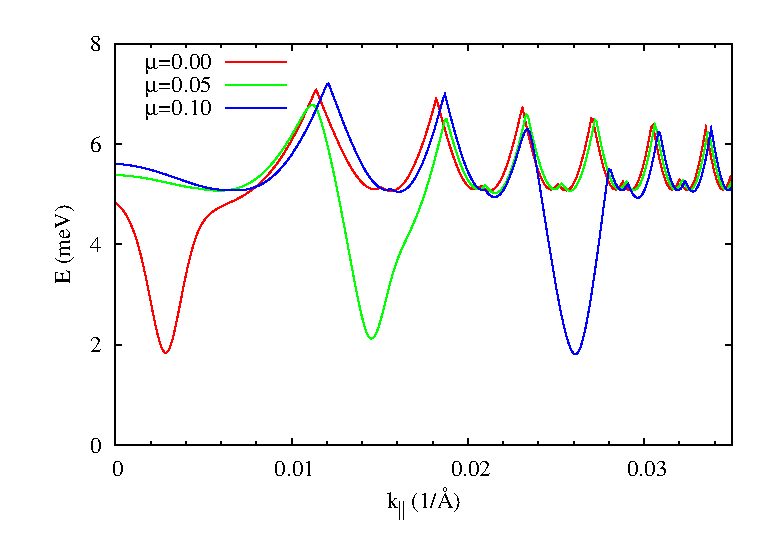
\includegraphics[width=3.4in]{disp-mu.eps}
\caption{The dispersion of the lowest energy level
for different $\mu$ (in eV). Other parameters
are the same as in Fig. \ref{lev-fk}, $L=160$nm and $\Delta_0\sim$5.2meV. Fu-Kane model
well describes the lowest energy mode. As $\mu$ is increased, 
$\Delta_s$ and $v_s$ stay roughly the same, while $\mu_s$ scales
linearly with $\mu$.
}\label{lev-chem}
\end{figure}
%%%%%%%%%%%%%%%%%%%%%%%%%%

%%%%%%%%%%%%%%%%%%%%%%%%%%
\begin{figure}
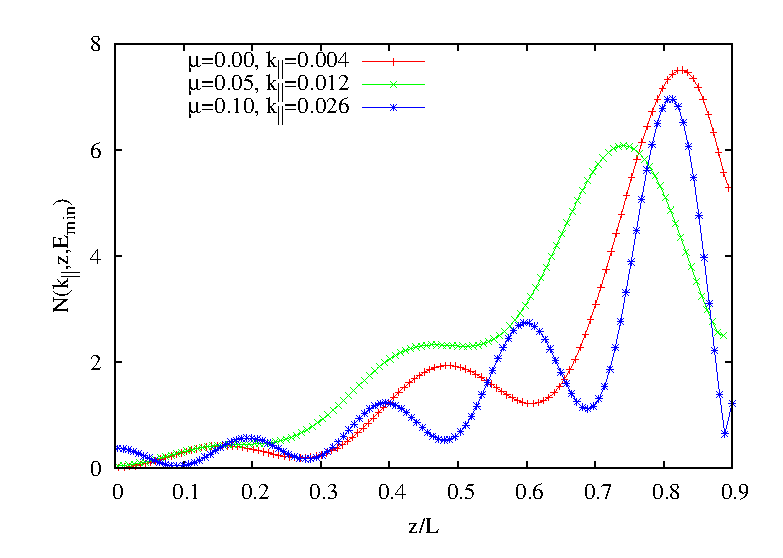
\includegraphics[width=3.4in]{spweight.eps}
\caption{The spectral function $N(k_\parallel,z,\omega)$ of the lowest 
energy level, $\omega=E_{min}$, shown in Fig. \ref{lev-chem}. 
The interface is at $z=0.9L$, $L$=160nm.
The spectral function oscillates rapidly with $z$, so only its envelope is plotted.
}\label{sp}
\end{figure}
%%%%%%%%%%%%%%%%%%%%%%%%%%

We have carried out similar analysis for superconductors with larger
coherence length. Fig. \ref{level-27} shows the evolution of
the sub-gap mode with $\mu$ for $\Delta_0=2.4$meV. In this case,
the values of $(\Delta_s,v_s,\mu_s)$ all varies with $\mu$. 
Superconductors with larger $\xi_0$ and smaller $\Delta_0$ are thus more
sensitive to changes in $\mu$ and other microscopic details near
the interface. The exact values of the effective parameters 
in the Fu-Kane model in general depend on such microscopic details.

%%%%%%%%%%%%%%%%%%%%%%%%%%
\begin{figure}
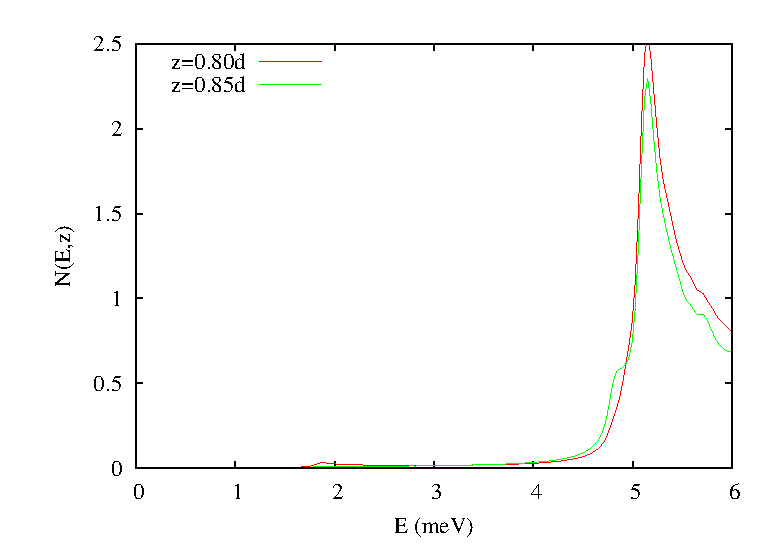
\includegraphics[width=3.4in]{dos.eps}
\caption{The local density of states $N(E,z)$
at $z=0.8d$ and $z=0.85d$ (the interface is at $z=0.9d$).
$\mu=0$, $L=160$nm, and $\Delta_0\sim$5.2meV. The subgap
states are due to the interface mode. A level broadening
$\sim 0.01\Delta_0$ is used.
}\label{dos}
\end{figure}
%%%%%%%%%%%%%%%%%%%%%%%%%%

%%%%%%%%%%%%%%%%%%%%%%%%%%
\begin{figure}
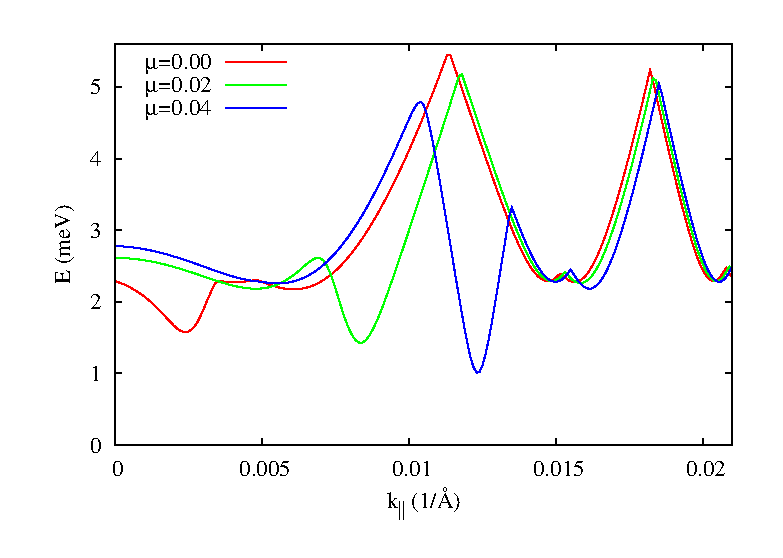
\includegraphics[width=3.4in]{spg27.eps}
\caption{The lowest energy level of an S-TI structure with $L=160$nm,
$d=0.9L$, $\Delta_0=2.4$meV. $\mu$ is the chemical potential of the TI and
measured in eV.}\label{level-27}
\end{figure}
%%%%%%%%%%%%%%%%%%%%%%%%%%

\section{Triplet Pair Correlations}

It is well known that in heterostructures of $s$-wave superconductors,
pairing correlations in other orbital channels, e.g. $p$-wave correlations, 
will be induced by scattering at the interfaces \cite{esch,tanaka}. For example,
inversion/reflection symmetry ($z\leftrightarrow -z$) is lost in an S-TI proximity 
structure, and the appearance of $p$-wave correlations seems natural from
 partial wave analysis. Moreover, scattering by a topological insulator is 
spin-active. The spin-orbit coupling inside a TI acts like a momentum-dependent
magnetic field to flip the electron spin and introduce different phase shifts
for spin up and down electrons. The scattering matrix has been worked out by us 
previously \cite{zhao}. Thus, a singlet $s$-wave Cooper pair can be converted into a pair
of electrons in spin-triplet state at the S-TI interface.
However, it is important to recall that by assumption attractive interaction only exists
(or is appreciable) in the $s$-wave channel. There is no binding force
to sustain a triplet Cooper pair or a triplet superconducting order parameter. 
%
Similar (but different) pairing correlations in superconductor-ferromagnet
hybrid structures have been extensively studied \cite{esch}. 
The appearance of $p$-wave correlations in S-TI systems
has been pointed out previously by Stanescu et al using a perturbative analysis \cite{stan}.

We focus on the equal-time pair correlation functions defined in Eq. \eqref{pair-corr}.
By exploiting the symmetry of the BdG Hamiltonian, Eq. \eqref{symm}, we are able to
find analytically the orbital structure of the triplet correlation functions. The unitary 
transformation Eq. \eqref{unit} yields
\begin{align}
u_{2\uparrow}(k_x,k_y)=u_{2\uparrow}(k_\parallel,0)e^{-i\varphi_k/2},\nn \\
u_{2\downarrow}(k_x,k_y)=u_{2\downarrow}(k_\parallel,0)e^{+i\varphi_k/2},\nn \\
v_{2\uparrow}(k_x,k_y)=v_{2\uparrow}(k_\parallel,0)e^{+i\varphi_k/2},\nn \\
v_{2\downarrow}(k_x,k_y)=v_{2\downarrow}(k_\parallel,0)e^{-i\varphi_k/2}. 
\end{align}
Using these relations, we find
\begin{align}
F_{\uparrow\uparrow}(\kperp,z)=F_{\uparrow\uparrow}(k_\parallel,z)e^{-i\varphi_k},\\
F_{\downarrow\downarrow}(\kperp,z)=F_{\downarrow\downarrow}(k_\parallel,z)e^{+i\varphi_k}.
\end{align}
Namely $F_{\uparrow\uparrow}$ ($F_{\downarrow\downarrow}$) has $p_x-ip_y$ ($p_x+ip_y$) orbital 
symmetry. Finally, the remaining triplet correlation function
\begin{equation}
\langle \psi_{2\uparrow}(\kperp,z) \psi_{2\downarrow} (-\kperp,z)+ \psi_{2\downarrow}(\kperp,z) \psi_{2\uparrow}(-\kperp,z)\rangle
\end{equation}
turns out to be zero. Note that the so-called odd-frequency paring correlations 
\cite{esch,tanaka,trip}, which vanishes in the equal-time limit, 
are also interesting in S-TI structures, but 
we will not discuss their behaviors here.

%%%%%%%%%%%%%%%%%%%%%%%%%%
\begin{figure}
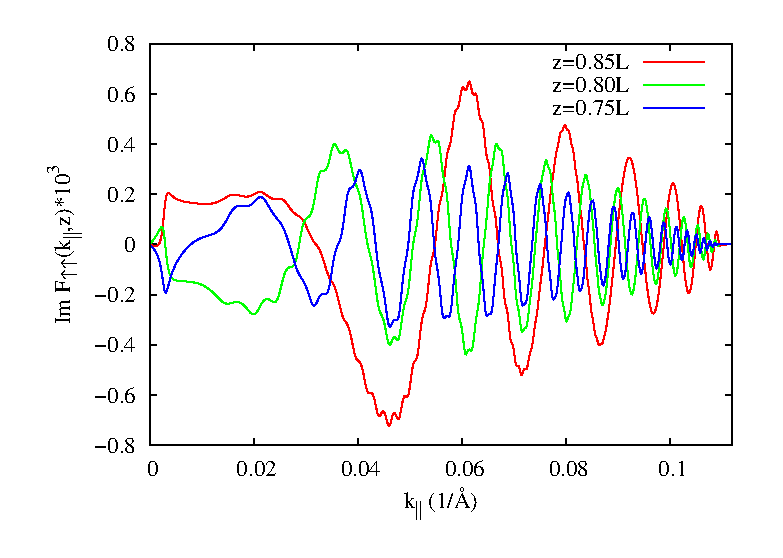
\includegraphics[width=3.4in]{pwave.eps}
\caption{The imaginary part of triplet pair correlation function 
$F_{\uparrow\uparrow}(k_\parallel,z)$. The S-TI interface is at
$d=0.9L$. $\mu=0$, $L=160$nm, $\Delta_0=5.2$meV.
}\label{pw}
\end{figure}
%%%%%%%%%%%%%%%%%%%%%%%%%%

We find that $F_{\uparrow\uparrow}(k_\parallel,z)$ is 
purely imaginary and identical to $F_{\downarrow\downarrow}(k_\parallel,z)$.
The results for $\mu=0$, $L=160$nm, $d=0.9L$, $\Delta_0=5.2$meV are plotted
in Fig. \ref{pw}. $F_{\uparrow\uparrow}$ vanishes at $k_\parallel=0$
as well as for large $k_\parallel$, namely when $k_\parallel>\sqrt{(E_F+\omega_D+M)/B_2}$.
This is consistent with lack of pairing in both limits. 
The behavior of $F_{\uparrow\uparrow}$ for small $k_\parallel$
is illustrated in Fig. \ref{pw-cu} for $\mu=0$, $L=300$nm, $d=0.95L$, 
$\Delta_0=0.6$meV. As comparison, we also plotted the singlet
 pair correlation function 
\begin{equation}
F_{\uparrow\downarrow}(\mathbf{k}_\parallel,z)=\sum'_n u_{n,2\uparrow}(\mathbf{k}_\parallel,z)
v^*_{n,2\downarrow}(-\mathbf{k}_\parallel,z)
\end{equation}
which is $s$-wave and purely real.

%%%%%%%%%%%%%%%%%%%%%%%%%%
\begin{figure}
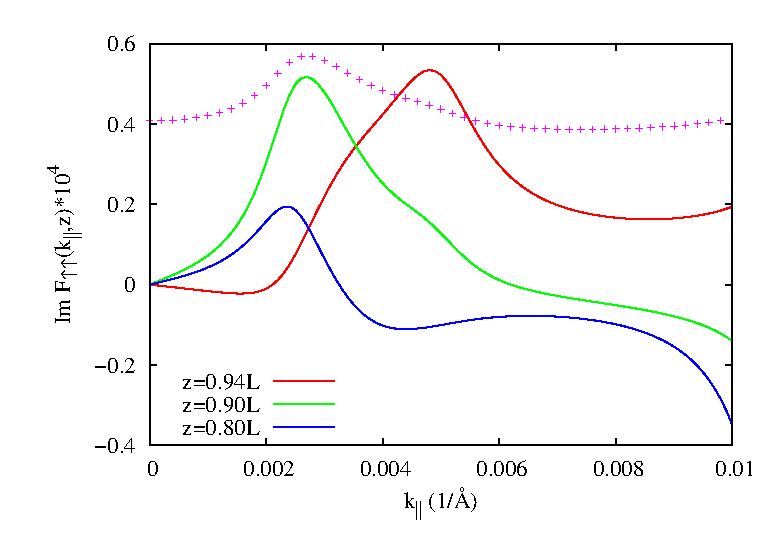
\includegraphics[width=3.4in]{pw-cu.eps}
\caption{The imaginary part of 
$F_{\uparrow\uparrow}(k_\parallel,z)$. $\mu=0$, $L=300$nm, $d=0.95L$, $\Delta_0=0.6$meV.
As comparison, the data points show the singlet pair correlation function 
$F_{\uparrow\downarrow}(k_\parallel,z=0.9L)/3$.
}\label{pw-cu}
\end{figure}
%%%%%%%%%%%%%%%%%%%%%%%%%%

\section{Summary and Outlook}
In summary, we have investigated the proximity effect between an $s$-wave superconductor
and a topological insulator using a microscopic continuum model. 
Strong coupling between the two materials renders the surface state of TI a less 
useful concept for this problem.
Our focus has been on the various modifications to superconductivity by the presence of TI. 
These include the suppression of the order parameter, the formation of interface modes
below the bulk superconducting gap, and the induction of triplet pairing correlations.
It is gratifying to see the Fu-Kane effective model emerges in the low energy sector
albeit with a set of renormalized parameters. Our results are complementary to
previous theoretical work on the proximity effect \cite{f-k,stan} and confirm the validity
of the Fu-Kane model.

We made a few simplifying assumptions in our calculation. The superconductor is described 
by a two-band model with the valence band well below the Fermi level. Since only 
electrons near the Fermi surface are relevant for weak coupling superconductivity, we 
believe our main results are general. As idealizations, the chemical 
potential, the spin-orbit coupling, and the attractive interaction are assumed to be 
step functions with a sudden jump at the interface. 
More elaborate and realistic models can be considered within the framework of BdG equations.
For example, one can add a tunneling barrier between S and TI, 
or include a Rashba-type spin-orbit coupling term 
(due to the gradient of chemical potential) at the interface. We will not 
pursuit these generalizations here.
Finally, the approach outlined here can be straightforwardly applied to 
study non-Abelian superconductivity in other superconductor-semiconductor
heterostructures where spin-orbit coupling also plays a significant role
\cite{roman,maryland,jason,mao1,mao2}.



\chapter{Josephson Junction on TI Surface}
\section{Introduction}
The study of topological insulators coupled with a superconductor has attracted much attention recently due to the implication of the possible existence of Majorana particles in such systems. Majoranas have several important reasons for their study, which include Topological Quantum computation and the novelty of being a particle that is its own antiparticle.

It has been proposed that an s-wave superconductor inducing superconductivity through proximity effect onto the surface of a TI can be host to Majorana particles in a vortex core interface of such a junction. In addition, a Josephson junction where the can also be host to 
such Majorana particles, as long as the Josephson phase between the the leads of the junction is $\pi$. Experimentally, it is a current challenge to acheive the Josephson $\pi$ junction, but progress has been made. Though this is a critical issue in developing such a structure, we proceed that it may be possible in the future. 
\section{Model and Basic Equations}

 %%%%%%%%%%%%%%%%%%%%%%%%%%
\begin{figure}
\center
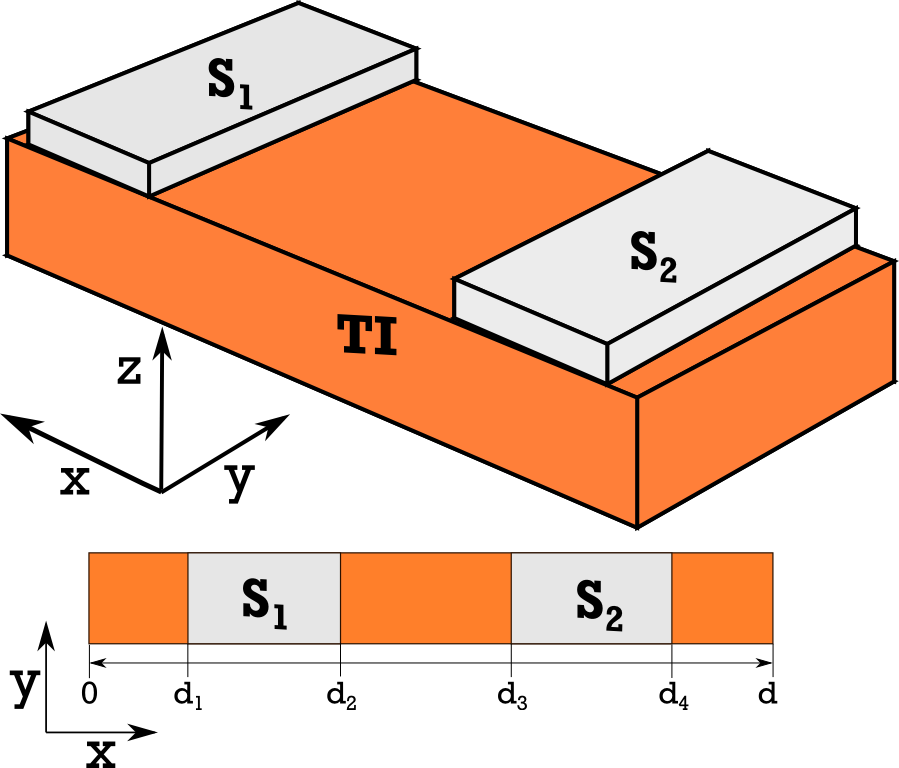
\includegraphics[width=3in]{setup.png}
\caption{(color online) Schematic (not to scale) of superconducting Josephson junction. S$_1$ and S$_2$ are the two superconducting leads that have phases of zero and $\pi$ respectively. 
}\label{setup}
\end{figure}
%%%%%%%%%%%%%%%%%%%%%%%%%%

We start with the physical model of our system as shown in fig.1. The system is restricted to the 2D surface of the TI where portions of the surface are in contact with an S-wave superconductor.  This proximity-induced superconductivity is modeled by the familiar Dirac-Bogoliubov-de Gennes Hamiltonian,
\begin{eqnarray}
&\mathcal{H}=\left(
\begin{array}{cc}
h_{+}  &  \hat{\Delta} \\
\hat{\Delta}^\dagger  &   h_{-}
\end{array}\label{fkmodel}
\right),&
\end{eqnarray}
where
\begin{eqnarray}
&h_{\pm}= -i\hbar  v_F (\sigma_x\partial_x \pm \sigma_y \partial_y) \mp \mu(x),&\\
&\hat{\Delta}= i\sigma_y  \Delta(x).&
\end{eqnarray}
 In the x-direction we have open boundary conditions and periodic boundary conditions in the y-direction, leading to plane wave ($exp({i k_y x})$) solutions, with $k_y$ as a good quantum number. $\Delta(x)$ is the spacially dependent order parameter.  $\mu(x)$ is the spacially dependent chemical potential, $v_F$ is the Fermi velocity, and $\sigma_i$ are the Pauli matrices. 

It is restriced to zero in the regions with where the superconductor is not in contact through a Heaviside stepfunction. $\phi_i$ are the phases of the superconductor order parameters of the two superconductor leads. In this setup we restrict the phase difference between the two superconducting  $\phi$ to be either 0 or $\pi$, otherwise we would have to consider possible super-current flow across the surface.

The basis,
\begin{equation}
%\left ( {\bf u} _{n\uparrow}(k_y, x),  {\bf u}_{n\downarrow}(k_y, x),  {\bf v}_{n\uparrow}(k_y, x), {\bf v}_{n\downarrow}(k_y, x) \right )^T,
\psi_n=\left ( { u} _{n\uparrow},  { u}_{n\downarrow},  { v}_{n\uparrow}, { v}_{n\downarrow} \right )^T,
\end{equation} 
which satisfies $ \mathcal{H}\psi_n=\epsilon_n \psi_n, $ represents the BdG particle ($u_\sigma (k_y, x)$), and hole ($v_\sigma (k_y, x)$) spatial wave amplitudes with their respective spins. For berevity the BdG index n will be supressed from here on.

We note the form of $h_{\pm}$ is derived from the TI k-space surface Hamiltonian, $H(k)=\hbar v_F \vec{\sigma}\cdot\vec{k}-\mu$, and its Time-reversed hole equivelent, $-H^*(-k)=\hbar v_F\vec{\sigma}^{\ast}\cdot\vec{k}+\mu$ by performing a Pierls substitution from k-space to real space ($k_i\rightarrow -i \partial_i$). We write the chemical potential as a spatially-dependent expression 
\begin{eqnarray}
\mu(x)=\left\{
\begin{array}{cc}
\mathcal{E}_F,&(d_1<x<d_2) \text{ or } (d_3<x<d_4)\\
\mu,& \text{elsewhere}\\
\end{array} \right .,
\end{eqnarray}

where 
%$\theta(x)$ is the Heaviside step function,  
$\mathcal{E}_F$ is the Fermi energy of the superconducting portion of the TI and $\mu$ is the tuned chemical potential of the metallic TI.


To self-consistently solve this system, we must start with an initial order parameter profile. We use a basic step function setup of the order parameter as: 
\begin{eqnarray}
\Delta(x)=\left\{
\begin{array}{cc}
\Delta_0,&(d_1<x<d_2)\\
\Delta_0 e^{i\phi},& (d_3<x<d_4)\\
0,& \text{elsewhere}\\
\end{array} \right .
\end{eqnarray}

Once an eigensystem is solved, we use the wavefunction to calculate the order parameter in the following gap equation
\begin{equation}
\Delta(x)=g(x)\int  d k_y \sum_n^\prime u_{n\uparrow}(k_y, x)v^*_{n\downarrow}(k_y, x)
\end{equation}\label{gap-eq}
\\
Where $g(x)$ is defined as a point contact pairing potential spatially as:

\begin{eqnarray}
g(x)=\left\{
\begin{array}{cc}
\mathcal{G}_0 [g_0],&(d_1<x<d_2) \text{ or } (d_3<x<d_4)\\
0,& \text{elsewhere}\\
\end{array} \right .
\end{eqnarray}

After calculating a new order parameter, it is fed back into the hamiltonian and the process is repeated until the difference between subsequent iterations of $\Delta(x)$ is under a desired small value.

In order to numerically solve this system, we employ the Fourier expansion technique by Valls et al and the authors. Details of this expansion are covered in refs. But the general approach is as follows.
We expand $u$, $v$, $\Delta$ as 
\begin{eqnarray}
u_{\sigma}(x)=\sum^N_{m=1} u_{m\sigma}\sqrt{2/d} \sin(k_m x)\\
v_{\sigma}(x)=\sum^N_{m=1} v_{m\sigma}\sqrt{2/d} \sin(k_m x)\\
\Delta(x)=\sum^N_{m=1} \Delta_{m}\sqrt{2/d} \sin(k_m x)
%u^n_{\sigma}(x)=\sum^N_{m=1} u^n_{m\sigma}\sqrt{2/d} \sin(k_m x)\\
%v^n_{\sigma}(x)=\sum^N_{m=1} v^n_{m\sigma}\sqrt{2/d} \sin(k_m x)\\
%\Delta(x)=\sum^N_{m=1} \Delta_{m}\sqrt{2/d} \sin(k_m x)
\end{eqnarray}
where %$\phi_m(x) = \sqrt{2/d} \sin(k_m x)$ and 
$k_m=m \pi /d$. The cutoff, N, is chosen as $\hbar  v_f k_m=\mathcal{E}_F + \omega_D$, where $\omega_d$, the Debye frequency, is taken to be about $.1 \mathcal{E}_F$.This basis expansion results in a 4N $\times$ 4N matrix Hamiltonian of:
\begin{eqnarray}
&\mathcal{H}=\left(
\begin{array}{cccc}
-\mu_{nm} &  \mathcal{K}^-_{nm} & 0 & \hat{\Delta}_{nm} \\
\mathcal{K}^+_{mn}  & -\mu_{nm}  & -\hat{\Delta}_{nm} & 0 \\
0 & -\hat{\Delta}_{nm}^\ast  & \mu_{nm} &  \mathcal{K}^+_{nm}\\
\hat{\Delta}_{nm}^\ast & 0 &  \mathcal{K}^-_{mn}  & \mu_{nm}
\end{array}\label{fkmodel}
\right),&
\end{eqnarray}
with
\begin{eqnarray}
\mathcal{K}^{\pm}_{nm}&=& -i\hbar  v_F (k_m B_{nm} \pm  k_y \delta_{nm}),\\
B_{nm} &=& \frac{2}{d}\int^d_0  \sin(k_n x) \cos(k_m x) dx\\
\mu_{nm}&=& \frac{2}{d}\int^d_0 \mu(x) \sin(k_n x) \sin(k_m x) dx\\
\hat{\Delta}_{nm}&=&  \frac{2}{d}\int^d_0 \Delta(x) \sin(k_n x) \sin(k_m x) dx
\end{eqnarray}
in the basis of
\begin{equation*}
\psi=  \left ( u_{n\uparrow1}...u_{n\uparrow N}, u_{n\downarrow1}...u_{n\downarrow N}, v_{n\uparrow1}...v_{n\uparrow N}, v_{n\downarrow1}...v_{n\downarrow N}, \right )^T,
\end{equation*} 

Using these techniques, we will solve two different types of SNS Josephson junction structures, one with a phase difference of $\phi=0$ and one with a phase difference of $\phi=\pi$. These two structures offer very different physics.

%%%%%%%%%%%%%%%%%%%%%%%%%%

\clearpage

\section{Energy Spectrum}

\begin{figure}[h]
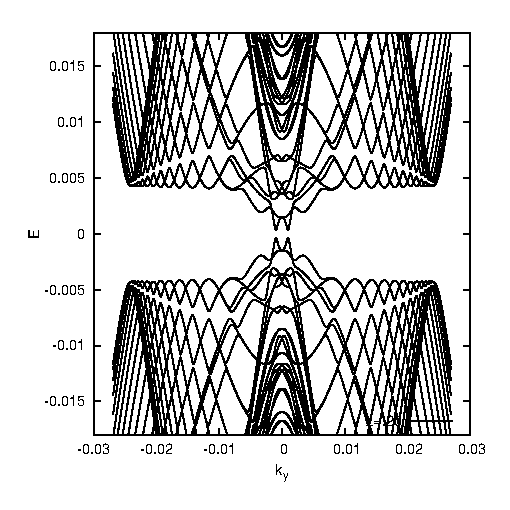
\includegraphics[width=3in]{energy_zero}
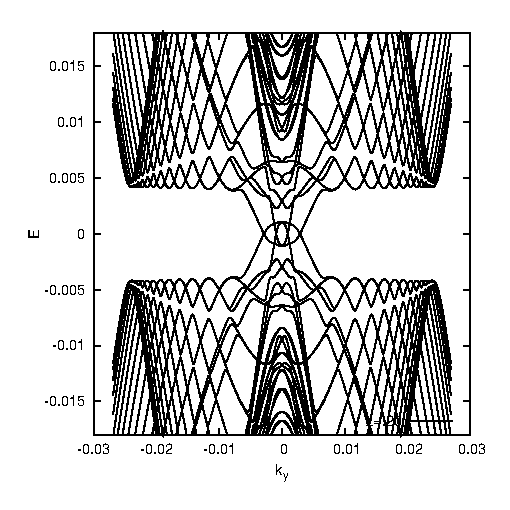
\includegraphics[width=3in]{energy_pi}
\caption{Energy spectrum of zero-bias (left) and pi-bias (right) junction. TI chemical potential is set to 5 meV. Energy in units of eV.
}\label{jj-energy}
\end{figure}

We calculate the energy spectrum as a function of of $k_y$ for the two types of junctions, zero-biased and $\pi$-biased. It is clear from figure \ref{jj-energy} that in the zero junction, the energy is fully gapped though there are subgap states that reside below the superconducting energy gap. In contrast, the $\pi$ junction, is {\it not} gapped but rather gapless. The symmetric nature of the energies in BdG formalism allows degenerate zero-energies to exist and these zero energies are the signature for Majorana modes. All spectrum calculations from $\mu$=0 to $\mu \approx \mathcal{E}_F $ are gapless (gapped) for the $\pi$ (zero) biased junction.

These gapless modes are the signature of a Topological phase transition. Just as the bulk of a TI is gapped and the surface is gapless, the same can be said about the "bulk" of a S-TI (zero phase) which goes through a phase transition ($\pi$ phase) into a Topological superconductor with gapless modes. 

\section{Order Parameter and Singlet Correlation}

\begin{figure}
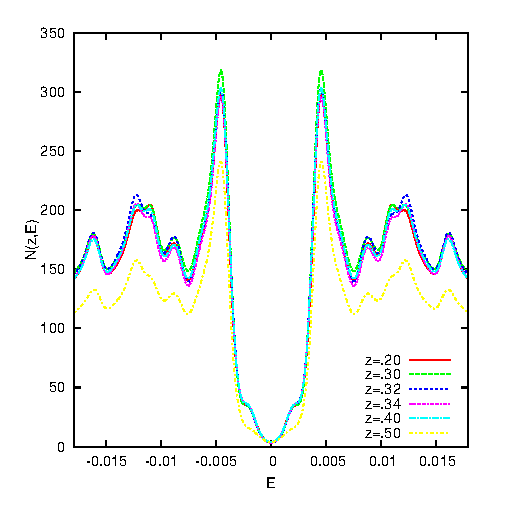
\includegraphics[width=3in]{dos_pi}
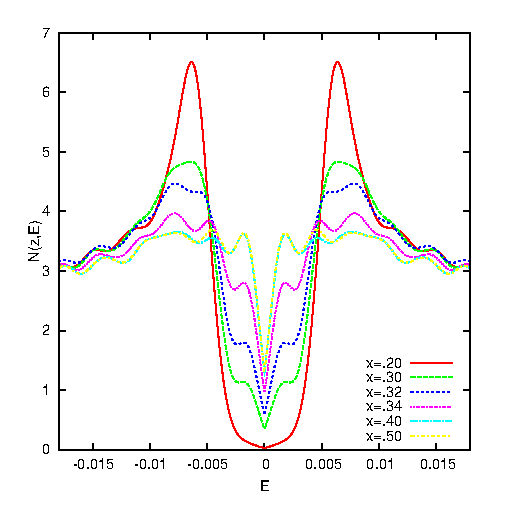
\includegraphics[width=3in]{dos_zero}
\caption{Local density of states at different positions in the heterostructure. Energy in units of eV.
}\label{ldos}
\end{figure}

In calculating the order parameter, $\Delta(x)$, from equation \ref{gap-eq} we also calculated the singlet correlation function, $F_{\uparrow\downarrow}(x)$ which is not restricted by the step function pairing potential, $g(x)$. This rescription simply sets the value of $\Delta(x)$ to zero in the non-superconducting regions of the structure. For berevity, we omit $\Delta(x)$ in favor of $F_{\uparrow\downarrow}(x)$, because physics is hidden in the non-superconducting region.

We can see that $F_{\uparrow\downarrow}(x)$ differs greatly between the two structures. In the $\pi$ junction we see a necessary drop in the magnitude to a zero value at the halfway mark of the junction. This singularity is required in order for the phase of to switch from 0 to $\pi$ from the left to the right side of the junction. This is the same story in the order parameter of a vortex, where the core of the vortex also has a zero value to allow the phase to "hop" from one side of the center to another. The zero junction on the other hand has a very interesting ``long-range" correlation. This is a by product of the spin-momnetum entanglement existing on the TI, which is a fabulous host to $F_{\uparrow\downarrow}(x)$ type of correlation. This story exists in the cousin of the TI, graphene, where Valls et al found a similar constant-like value for the correlation. 

\section{Local Density of States}
\begin{figure}
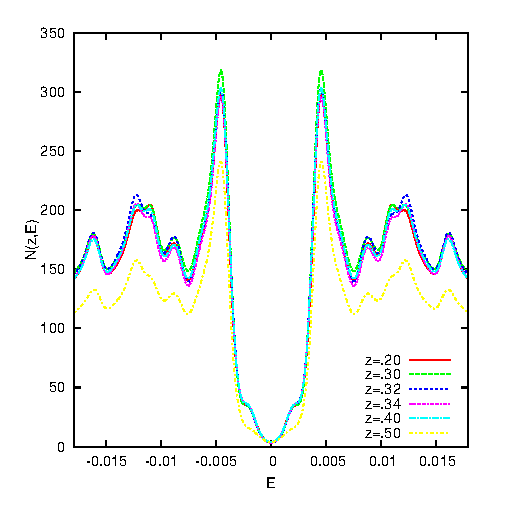
\includegraphics[width=3in]{dos_pi}
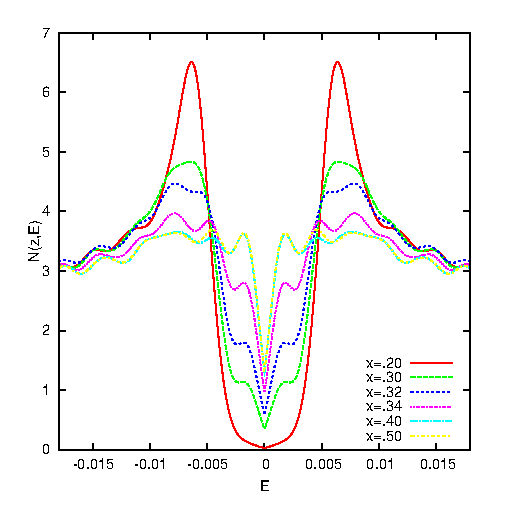
\includegraphics[width=3in]{dos_zero}
\caption{Local density of states at different positions in the heterostructure. Left (right) is the zero ($\pi$) biased junction. Energy in units of eV.
}\label{ldos-jj}
\end{figure}
Plotted in figure \ref{ldos-jj} are the local density of states of the two junction types with $\mu \approx \mathcal{E}_F$. It is evident from these plots that an emergence of states exist within the superconducting gap. 

\section{Spectral Function}
\begin{figure}
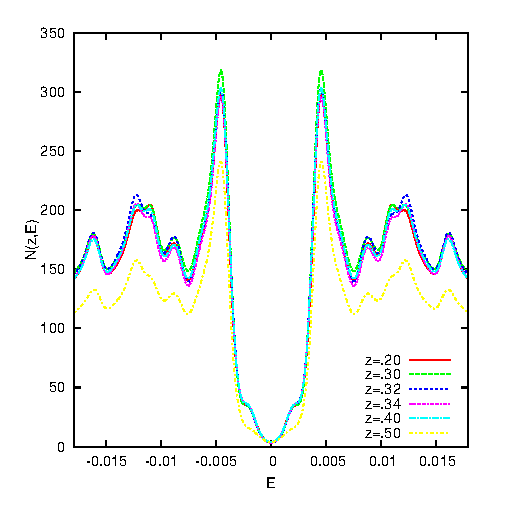
\includegraphics[width=3in]{dos_pi}
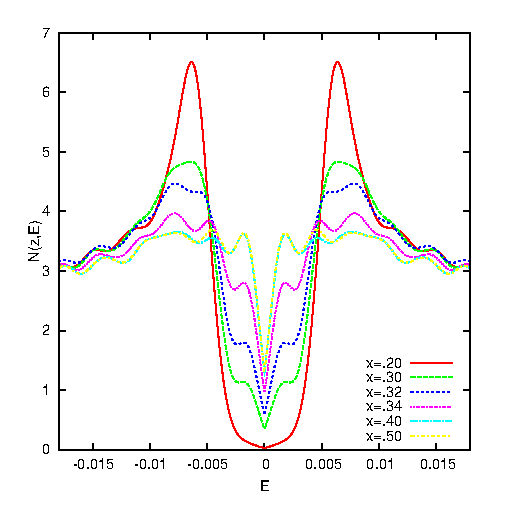
\includegraphics[width=3in]{dos_zero}
\caption{Local spectral function near the midpoint ($\approx .55$) of the heterostructure. Left (right) is the zero ($\pi$) biased junction. Energy in units of eV.
}\label{spectral-jj}
\end{figure}
Lastly, we show the local spectral function of the two structures. This shows the similar story that the energy spectrum told in regards to the gapped/gapless states. 
%%%%%%%%%%%%%%%%%%%%%%%%%%

\chapter{TI-FET: MOSFET with a Topological Insulator}
\section{Introduction}
\begin{figure}[h]
\center
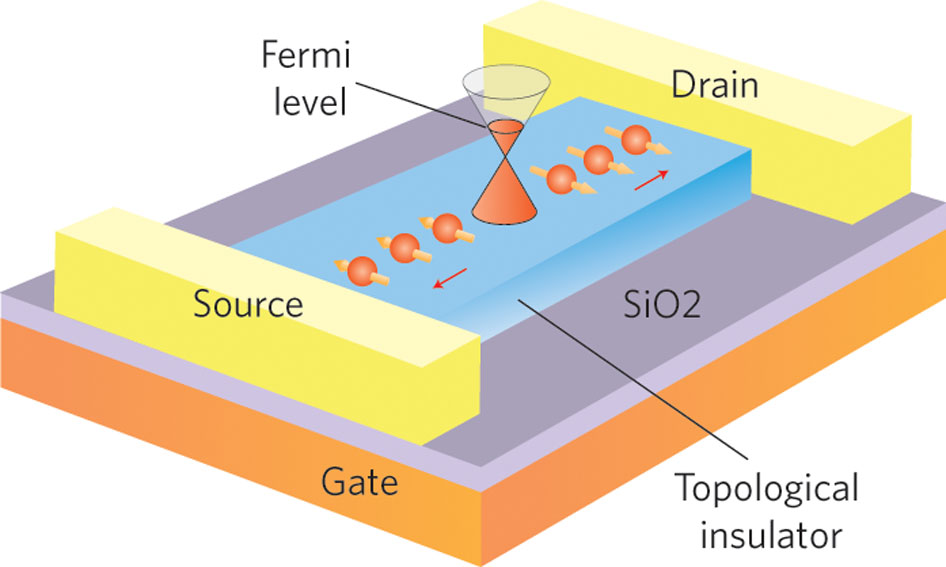
\includegraphics[width=5in]{tifet.jpg}
\caption{A proposed heterostructure that exploits the exotic surface states that differ from the bulk in a TI. 
}\label{tifet}
\end{figure}
In this chapter I present ideas proposed by Professor Qialang Li of the Electrical and Computer Engineering department. Professor Li is an expert at electronic device physics and has suggested to utilize a TI in a MOSFET type of structure as a floating gate. In addition it was proposed [need cite] to use a TI as a current channel to provide new characteristics of a transistor.  To give a proper overview of such ideas, I first present a quick introduction on how a MOSFET works, then I show two proposals of structures to be be built. Lastly, I will describe the general outline of how to simulate the physics of these structures to give insight in designing them.

\section{MOSFET}

\section{TI as the Floating Gate}

\section{TI as the current channel}

%\chapter{Topological Transitions in Non-Equilibrium Spin-Orbit-Coupled Cold Atoms}


\bibliographystyle{apsrev}
\begin{thebibliography}{29}


\bibitem{f-k} L. Fu and C. L. Kane,
Phys. Rev. Lett. 100, 096407 (2008)
\bibitem{r-g} N. Read and D. Green, Phys. Rev. B 61, 10267�10297 (2000)
\bibitem{qi-zhang}X.-L. Qi and S.-C. Zhang, arXiv:1008.2026
\bibitem{rmp} M. Z. Hasan and C. L. Kane, Rev. Mod. Phys. 82, 3045 (2010)
\bibitem{roman} R. M. Lutchyn, J. D. Sau, and S. Das Sarma,
Phys. Rev. Lett. 105, 077001 (2010)
\bibitem{maryland} J. D. Sau et al, Phys. Rev. B 82, 214509 (2010)
\bibitem{jason} J. Alicea, Phys. Rev. B 81, 125318 (2010)
\bibitem{mao1} L. Mao, and C. Zhang, Phys. Rev. B 82, 174506 (2010)
\bibitem{mao2} L. Mao, J. Shi, Q. Niu, and C. Zhang, arXiv:1010.0932 (2010)

\bibitem{yu} Y. Tanaka, T. Yokoyama, and N. Nagaosa, Phys. Rev. Lett. 103, 107002 (2009)
\bibitem{jacF} J. Linder, Y. Tanaka, T. Yokoyama, A. Sudbo, and N. Nagaosa,
Phys. Rev. B 81, 184525 (2010)

\bibitem{jacU} J. Linder, Y. Tanaka, T. Yokoyama, A. Sudbo, and N. Nagaosa,
 Phys. Rev. Lett. 104, 067001 (2010)

\bibitem{sca} B. Sacepe, J. B. Oostinga, J. Li, A. Ubaldini, N. J. G. Couto, E. Giannini, and A. F. Morpurgo,
arXiv:1101.2352 (2011)
\bibitem{march}M. Veldhorst et al, http://meetings.aps.org/Meeting
/MAR11/Event/143261;
D.M. Zhang et al, http://
meetings.aps.org/Meeting/MAR11/Event/143273

\bibitem{stan}T. D. Stanescu, J. D. Sau, R. M. Lutchyn, and S. Das Sarma,
Phys. Rev. B 81, 241310 (2010)
\bibitem{ann} A. M. Black-Schaffer, arXiv:1010.4625 (2010)

\bibitem{cu1} Y. S. Hor et al, Phys. Rev. Lett. 104, 057001 (2010)
\bibitem{cu2} L. A. Wray et al, Nature Physics 6, 855 (2010)
\bibitem{ando} M. Kriener, K. Segawa, Z. Ren, S. Sasaki, and Y. Ando,
Phys. Rev. Lett. 106, 127004 (2011)

\bibitem{zhang} H. Zhang et al, Nature Physics 5, 438 (2009)
\bibitem{band} W. Zhang, R. Yu, H.-J. Zhang, X. Dai, and Z. Fang, New J. Phys. 12, 065013 (2010)
\bibitem{gate}J. G. Checkelsky, Y. S. Hor, R. J. Cava, and N. P. Ong, arXiv:1003.3883
\bibitem{h-v}K. Halterman and O. T. Valls, Phys. Rev. B 65,  014509 (2001)
\bibitem{s-v}B. P. Stojkovic and O. T. Valls, Phys. Rev. B 47, 5922 (1993)
\bibitem{zhao}E. Zhao, C. Zhang, and M. Lababidi, Phys. Rev. B 82, 205331 (2010) 
\bibitem{toku}T. Tokuyasu, J. A. Sauls, and D. Rainer, Phys. Rev. B 38, 8823 (1988)
\bibitem{esch}M. Eschrig, T. L\"ofwander, T. Champel, J. C. Cuevas, J. Kopu, and G. Sch\"on,
J. Low Temp. Phys. 147, 457 (2007)
\bibitem{tanaka}A. A. Golubov, Y. Tanaka, Y Asano and Y Tanuma, J. Phys.: Condens. Matter 21, 164208 (2009)
\bibitem{trip}F. S. Bergeret, A. F. Volkov, and K. B. Efetov, Rev. Mod. Phys. 1321 (2005)




\end{thebibliography}
\end{document} 